% LaTeX source for ``Complexity and Computation''
% Copyright (c)  2011  Allen B. Downey.

% Permission is granted to copy, distribute, transmit and adapt
% this work under a Creative Commons
% Attribution-NonCommercial-ShareAlike 3.0 Unported License:
% http://creativecommons.org/licenses/by-nc-sa/3.0/

% If you are interested in distributing a commercial version of this
% work, please contact Allen B. Downey.

% The LaTeX source for this book is available from
% http://greenteapress.com/complexity
% http://code.google.com/p/complexity

% This book was typeset using LaTeX .  The illustrations were
% drawn in xfig.  All of these are free, open-source programs.

%%----------------------------------------------------------------

% How to compile this document:
% If your environment provides latex, makeindex, and dvips,
% the following commands should produce a Postscript version
% of the book.

%        latex book
%        makeindex book
%        latex book
%        dvips -o book.ps book

% You will also need the following (fairly standard) latex
% packages: url, epsfig, makeidx, fancyhdr

% This distribution also includes a Makefile that should
% compile both the Postscript and PDF versions of the book.

%%-----------------------------------------------------------------

\documentclass[10pt]{book}
\usepackage[width=5.5in,height=8.0in,
  hmarginratio=3:2,vmarginratio=1:1]{geometry}

\usepackage{url}
\usepackage{fancyhdr}
\usepackage{graphicx}
\usepackage{amsmath, amsthm, amssymb}
\usepackage{exercise}
\usepackage{makeidx}
\usepackage{setspace}
\usepackage{hevea}
\usepackage{upquote}

\usepackage{soul}

\newcommand{\thetitle}{Complexity and Computation}
\newcommand{\theversion}{1.0.3}

% these styles get translated in CSS for the HTML version
\newstyle{a:link}{color:purple;}
\newstyle{p+p}{margin-top:1em;margin-bottom:1em}
\newstyle{img}{border:0px}

% change the arrows in the HTML version
\setlinkstext
  {\imgsrc[ALT="Previous"]{back.png}}
  {\imgsrc[ALT="Up"]{up.png}}
  {\imgsrc[ALT="Next"]{next.png}}

\makeindex

\begin{document}

\frontmatter

% LATEXONLY

\input{latexonly}

\newtheorem{ex}{Exercise}[chapter]

\begin{latexonly}

\renewcommand{\blankpage}{\thispagestyle{empty} \quad \newpage}

%\blankpage
%\blankpage

% TITLE PAGES FOR LATEX VERSION

%-half title--------------------------------------------------
\thispagestyle{empty}

\begin{flushright}
\vspace*{2.0in}

\begin{spacing}{3}
{\huge \thetitle}
\end{spacing}

\vspace{0.25in}

Version \theversion

\vfill

\end{flushright}

%--verso------------------------------------------------------

\blankpage
\blankpage
%\clearemptydoublepage
%\pagebreak
%\thispagestyle{empty}
%\vspace*{6in}

%--title page--------------------------------------------------
\pagebreak
\thispagestyle{empty}

\begin{flushright}
\vspace*{2.0in}

\begin{spacing}{3}
{\huge \thetitle}
\end{spacing}

\vspace{0.25in}

Version \theversion

\vspace{1in}


{\Large
Allen Downey\\
}


\vspace{0.5in}

{\Large Green Tea Press}

{\small Needham, Massachusetts}

%\includegraphics[width=1in]{figs/logo1.eps}
\vfill

\end{flushright}


%--copyright--------------------------------------------------
\pagebreak
\thispagestyle{empty}

{\small
Copyright \copyright ~2011 Allen Downey.


Printing history:

\begin{description}

\item[Fall 2008:] First edition.

\item[Fall 2011:] Second edition.

\end{description}

\vspace{0.2in}

\begin{flushleft}
Green Tea Press       \\
9 Washburn Ave \\
Needham MA 02492
\end{flushleft}

Permission is granted to copy, distribute, transmit and adapt
this work under a Creative Commons
Attribution-NonCommercial-ShareAlike 3.0 Unported License:
\url{http://creativecommons.org/licenses/by-nc-sa/3.0/}.

If you are interested in distributing a commercial version of this
work, please contact Allen B. Downey.

The original form of this book is \LaTeX\ source code.  Compiling this
\LaTeX\ source has the effect of generating a device-independent
representation of the book, which can be converted to other formats
and printed.

The \LaTeX\ source for this book is available from

\begin{verbatim}
      http://greenteapress.com/complexity
      http://code.google.com/p/complexity
\end{verbatim}

This book was typeset using \LaTeX .  The illustrations were
drawn in xfig.

The cover photo is courtesy of {\tt blmurch}, and is available
under a free license from
\url{http://www.flickr.com/photos/blmurch/2034678924/sizes/l/in/photostream/}.

\vspace{0.2in}

} % end small

\end{latexonly}


% HTMLONLY

\begin{htmlonly}

% TITLE PAGE FOR HTML VERSION

{\Large \thetitle}

{\large Allen B. Downey}

Version \theversion

\setcounter{chapter}{-1}

\end{htmlonly}

\chapter{Preface}

This book is about data structures and algorithms, intermediate
programming in Python, computational modeling and
the philosophy of science:

\begin{description}

\item[Data structures and algorithms:] A data structure is a
  collection of data elements organized in a way that supports
  particular operations.  For example, a Python dictionary organizes
  key-value pairs in a way that provides fast mapping from keys to
  values, but mapping from values to keys is slower.
\index{data structure}
\index{algorithm}

An algorithm is a mechanical process for performing a computation.
Designing efficient programs often involves the co-evolution of data
structures and the algorithms that use them.  For example, in the
first few chapters I will present graphs, data structures that
implement graphs, and graph algorithms based on those data structures.
\index{graph algorithm}

\item[Python programming:] This book picks up where {\em Think Python}
  leaves off.  I assume that you have read that book or have
  equivalent knowledge of Python.  I try to emphasize fundamental ideas
  that apply to programming in many languages, but along the way you
  will learn some useful features that are specific to Python.
\index{Think Python@{\em Think Python}}

\item[Computational modeling:] A model of a system is a simplified
  description of a system used for simulation or analysis.
  Computational models are designed to take advantage of cheap, fast
  computation.
\index{modeling}

\item[Philosophy of science:] The models and results in this book
  raise questions relevant to the philosophy of science,
  including the nature of scientific laws, theory choice, realism and
  instrumentalism, holism and reductionism, and epistemology.
\index{philosophy}

\end{description}

There are two kinds of computational models:

\begin{description}

\item[Continuous:] Many computational models compute approximate
  solutions to equations that are continuous in space and time.  For
  example, to compute the trajectory of a planet, you could describe
  planetary motion using differential equations and then compute the
  position of the planet at discrete points in time.
\index{continuous model}

The fields of numerical methods and scientific computing
tend to focus on these kinds of models.
\index{numerical methods}
\index{scientific computing}

\item[Discrete:] Discrete models include graphs, cellular automata,
  and agent-based models.  They are often characterized by structure,
  rules and transitions rather than by equations.  They tend to be
  more abstract than continuous models; in some cases there is no
  direct correspondence between the model and a physical system.
\index{discrete model}

\end{description}

Complexity science is an interdisciplinary field---at the intersection
of mathematics, computer science and natural science---that focuses on
discrete models of physical systems.
\index{complexity science}

And that's what this book is about.


Allen B. Downey \\
Needham MA\\

Allen Downey is a Professor of Computer Science at
the Franklin W. Olin College of Engineering.




\section*{Contributor List}

\index{contributors}

If you have a suggestion or correction, please send email to
{\tt downey@greenteapress.com}.  If I make a change based on your
feedback, I will add you to the contributor list
(unless you ask to be omitted).
\index{contributors}

If you include at least part of the sentence the
error appears in, that makes it easy for me to search.  Page and
section numbers are fine, too, but not quite as easy to work with.
Thanks!

\small

\begin{itemize}

\item Richard Hollands pointed out several typos.

\item John Harley, Jeff Stanton, Colden Rouleau and
Keerthik Omanakuttan are Computational Modeling students who
pointed out typos.

\item Muhammad Najmi bin Ahmad Zabidi caught some typos.

\item Phillip Loh, Corey Dolphin, Noam Rubin and Julian Ceipek
found typos and made helpful suggestions.

\item Jose Oscar Mur-Miranda found several typos.

% ENDCONTRIB

\end{itemize}

\normalsize

\clearemptydoublepage

% TABLE OF CONTENTS
\begin{latexonly}

\tableofcontents

\clearemptydoublepage

\end{latexonly}

% START THE BOOK
\mainmatter


\chapter{Graphs}

\section{What's a graph?}

To most people a graph is a visual representation of a data set, like
a bar chart or an EKG.  That's not what this chapter is about.
\index{graph}

In this chapter, a {\bf graph} is an abstraction used to
model a system that contains discrete, interconnected elements.  The
elements are represented by {\bf nodes} (also called {\bf vertices})
and the interconnections are represented by {\bf edges}.
\index{node}
\index{edge}
\index{vertex}

For example, you could represent a road map with one node for each
city and one edge for each road between cities.  Or you could
represent a social network using one node for each person, with an
edge between two people if they are ``friends'' and no edge otherwise.
\index{road network}
\index{social network}

In some graphs, edges have different lengths (sometimes
called ``weights'' or ``costs'').  For example, in a road map, the
length of an edge might represent the distance between
two cities, or the travel time, or bus fare.
In a social network there might be different kinds of
edges to represent different kinds of relationships: friends,
business associates, etc.
\index{edge weight}
\index{weight}

Edges may be {\bf undirected}, if they represent a relationship
that is symmetric, or {\bf directed}.  In a social network,
friendship is usually symmetric: if $A$ is friends with $B$ then
$B$ is friends with $A$.  So you would probably represent friendship
with an undirected edge.  In a road map, you would probably represent
a one-way street with a directed edge.
\index{directed graph}
\index{undirected graph}

Graphs have interesting mathematical properties, and
there is a branch of mathematics called {\bf graph theory}
that studies them.
\index{graph theory}

Graphs are also useful, because there are many real world
problems that can be solved using {\bf graph algorithms}.
For example, Dijkstra's shortest path algorithm is an efficient
way to find the shortest path from a node to all
other nodes in a graph.  A {\bf path} is a sequence of nodes
with an edge between each consecutive pair.
\index{graph algorithm}
\index{path}

Sometimes the connection between a real world problem and
a graph algorithm is obvious.  In the road map example, it is
not hard to imagine using a shortest path algorithm to find
the route between two cities that minimizes distance (or time,
or cost).
\index{shortest distance}

In other cases it takes more effort to represent a problem in a form
that can be solved with a graph algorithm, and then interpret the
solution.
\index{problem formulation}

For example, a complex system of radioactive decay
can be represented by a
graph with one node for each nuclide (type of atom) and an edge
between two nuclides if one can decay into the other.  A path in this
graph represents a decay chain.
See \url{wikipedia.org/wiki/Radioactive_decay}.
\index{radioactive decay}
\index{decay chain}

The rate of decay between two nuclides is characterized by a decay
constant, $\lambda$, measured in becquerels (Bq) or decay events per
second.  You might be more familiar with half-life, $t_{1/2}$, which
is the expected time until half of a sample decays.  You can convert
from one characterization to the other using the relation $t_{1/2} =
\ln 2 / \lambda$.
\index{half life}
\index{becquerel}

In our best current model of physics, nuclear decay is a fundamentally
random process, so it is impossible to predict when an atom will
decay.  However, given $\lambda$, the probability that an atom will
decay during a short time interval $dt$ is $\lambda dt$.
\index{random process}

In a graph with multiple decay chains, the probability of a
given path is the product of the probabilities of each decay
process in the path.

Now suppose you want to find the decay chain with the highest
probability.  You could do it by assigning each edge a ``length'' of
$-\log \lambda$ and using a shortest path algorithm.  Why?  Because the
shortest path algorithm adds up the lengths of the edges, and adding
up log-probabilities is the same as multiplying probabilities.  Also,
because the logarithms are negated, the smallest sum corresponds to
the largest probability.  So the shortest path corresponds to the most
likely decay chain.

This is an example of a common and useful process in applying
graph algorithms:
\index{applying graph algorithm}

\begin{description}

\item[Reduce] a real-world problem to an instance of a graph
problem.

\item[Apply] a graph algorithm to compute the result efficiently.

\item[Interpret] the result of the computation in terms of a
solution to the original problem.

\end{description}

We will see other examples of this process soon.

\begin{ex}

Read the Wikipedia page about graphs at
\url{http://en.wikipedia.org/wiki/Graph_(mathematics)}
and answer the following questions:

\begin{enumerate}

\item What is a simple graph?  In the rest of this section,
we will be assuming that all graphs are simple graphs.  This
is a common assumption for many graph algorithms---so
common it is often unstated.
\index{simple graph}

\item What is a regular graph?  What is a complete graph?  Prove
that a complete graph is regular.
\index{regular graph}
\index{complete graph}

\item What is a path?  What is a cycle?
\index{path}
\index{cycle}

\item What is a forest?  What is a tree?  Note: a graph
is {\bf connected} if there is a path from every node to
every other node.
\index{forest}
\index{connected graph}

\end{enumerate}

\end{ex}



\section{Representing graphs}

Graphs are usually drawn with squares or circles for nodes and lines
for edges.  In the example below, the graph on the left represents
a social network with three people.
\index{representing graphs}

%A set of nodes like this,
%where each node is connected to all of the others, is called
%a {\bf clique} (pronounced ``cleek'').

\beforefig
\centerline{\includegraphics[width=5.5in]{figs/graph_examples.eps}}
\afterfig

In the graph on the right, the weights of the edges are the
approximate travel times, in hours, between cities in the northeast
United States.  In this case the placement of the nodes corresponds
roughly to the geography of the cities, but in general the layout
of a graph is arbitrary.
\index{graph layout}

To implement graph algorithms, you have to figure
out how to represent a graph in the form of a data structure.
But to choose the best data structure, you have to know which
operations the graph should support.
\index{data structure}

To get out of this chicken-and-egg problem, I am going to present
a data structure that is a good choice for many graph algorithms.
Later we will come back and evaluate its pros and cons.

Here is an implementation of a graph as a dictionary of dictionaries:
\index{dictionary}
\index{nested dictionary}
\index{Graph@{\tt Graph}}

\begin{verbatim}
class Graph(dict):
    def __init__(self, vs=[], es=[]):
        """create a new graph.  (vs) is a list of vertices;
        (es) is a list of edges."""
        for v in vs:
            self.add_vertex(v)

        for e in es:
            self.add_edge(e)

    def add_vertex(self, v):
        """add (v) to the graph"""
        self[v] = {}

    def add_edge(self, e):
        """add (e) to the graph by adding an entry in both directions.

        If there is already an edge connecting these Vertices, the
        new edge replaces it.
        """
        v, w = e
        self[v][w] = e
        self[w][v] = e
\end{verbatim}

The first line declares that {\tt Graph} inherits from the built-in
type {\tt dict}, so a Graph object has all the methods and operators
of a dictionary.
\index{inheritance}

More specifically, a Graph is a dictionary that maps from
a Vertex $v$ to an inner dictionary that maps from a Vertex $w$
to an Edge that connects $v$ and $w$.  So if {\tt g} is a graph,
{\tt g[v][w]} maps to an Edge if there is one and raises
a {\tt KeyError} otherwise.
\index{vertex}
\index{edge}

\verb"__init__" takes a list of vertices and a list of
edges as optional parameters.  If they are provided, it calls
\verb"add_vertex" and \verb"add_edge" to add the vertices and edges to
the graph.
\index{optional parameter}

Adding a vertex to a graph means making an entry for it in the
outer dictionary.  Adding an edge makes two entries, both pointing
to the same Edge.  So this implementation represents an undirected
graph.
\index{directed edge}
\index{undirected edge}

Here is the definition for {\tt Vertex}:
\index{Vertex@{\tt Vertex}}

\begin{verbatim}
class Vertex(object):
    def __init__(self, label=''):
        self.label = label

    def __repr__(self):
        return 'Vertex(%s)' % repr(self.label)

    __str__ = __repr__
\end{verbatim}

A Vertex is just an object that has a label attribute.  We can
add attributes later, as needed.
\index{label}

\verb"__repr__" is a special function that returns a string
representation of an object.  It is similar to \verb"__str__" except
that the return value from \verb"__str__" is intended to be readable
for people, and the return value from \verb"__repr__" is supposed to
be a legal Python expression.
\index{repr@{\tt \_\_repr\_\_}}
\index{str@{\tt \_\_str\_\_}}
\index{str@{\tt str}}
\index{repr@{\tt repr}}

The built-in function {\tt str} invokes \verb"__str__" on
an object; similarly the built-in function {\tt repr} invokes
\verb"__repr__".

In this case \verb"Vertex.__str__" and \verb"Vertex.__repr__" refer to
the same function, so we get the same string either way.

Here is the definition for {\tt Edge}:
\index{Edge@{\tt Edge}}

\begin{verbatim}
class Edge(tuple):
    def __new__(cls, *vs):
        return tuple.__new__(cls, vs)

    def __repr__(self):
        return 'Edge(%s, %s)' % (repr(self[0]), repr(self[1]))

    __str__ = __repr__
\end{verbatim}

{\tt Edge} inherits from the built-in type {\tt tuple}
and overrides the \verb"__new__" method.  When you invoke
an object constructor, Python invokes \verb"__new__" to create
the object and then \verb"__init__" to initialize the attributes.
\index{tuple}
\index{new@{\tt \_\_new\_\_}}
\index{init@{\tt \_\_init\_\_}}

For mutable objects it is most common to override
\verb"__init__" and use the default implementation of
\verb"__new__", but because Edges inherit from {\tt tuple}, they
are immutable, which means that you can't modify the elements
of the tuple in \verb"__init__".
\index{mutable objects}
\index{immutable objects}

By overriding \verb"__new__", we can use the {\tt *} operator to
gather the parameters and use them to initialize the elements of
the tuple.  A precondition of this method is that there should
be exactly two arguments.  A more careful implementation would
check.
\index{override}
\index{gather operator}
\index{precondition}

Here is an example that creates two vertices and an edge:

\begin{verbatim}
    v = Vertex('v')
    w = Vertex('w')
    e = Edge(v, w)
    print e
\end{verbatim}

Inside \verb"Edge.__str__" the term {\tt self[0]} refers
to {\tt v} and {\tt self[1]} refers to {\tt w}.  So the output
when you print {\tt e} is:

\begin{verbatim}
Edge(Vertex('v'), Vertex('w'))
\end{verbatim}

Now we can assemble the edge and vertices into a graph:

\begin{verbatim}
    g = Graph([v, w], [e])
    print g
\end{verbatim}

The output looks like this (with a little formatting):

\begin{verbatim}
{Vertex('w'): {Vertex('v'): Edge(Vertex('v'), Vertex('w'))},
 Vertex('v'): {Vertex('w'): Edge(Vertex('v'), Vertex('w'))}}
\end{verbatim}

We didn't have to write \verb"Graph.__str__"; it is inherited
from {\tt dict}.
\index{inheritance}


\begin{ex}

In this exercise you write methods that will be
useful for many of the Graph algorithms that are coming up.
\index{graph methods}

\begin{enumerate}

\item Download \url{thinkcomplex.com/GraphCode.py}, which
  contains the code in this chapter.  Run it as a script and make sure
  the test code in {\tt main} does what you expect.

\item Make a copy of {\tt GraphCode.py} called {\tt Graph.py}.  Add
  the following methods to {\tt Graph}, adding test code as you go.

\item Write a method named \verb"get_edge" that takes two vertices and
  returns the edge between them if it exists and {\tt None} otherwise.
  Hint: use a {\tt try} statement.

\item Write a method named \verb"remove_edge" that takes an edge and
  removes all references to it from the graph.

\item Write a method named {\tt vertices} that returns a list of the
  vertices in a graph.

\item Write a method named {\tt edges} that returns a list of edges in
  a graph.  Note that in our representation of an undirected graph
  there are two references to each edge.

\item Write a method named \verb"out_vertices" that takes a Vertex and
  returns a list of the adjacent vertices (the ones connected to the
  given node by an edge).

\item Write a method named \verb"out_edges" that takes a Vertex and
  returns a list of edges connected to the given Vertex.

\item Write a method named \verb"add_all_edges" that starts with an
  edgeless Graph and makes a complete graph by adding edges between
  all pairs of vertices.

\end{enumerate}

Test your methods by writing test code and checking the output.  Then
download \url{thinkcomplex.com/GraphWorld.py}.  GraphWorld is
a simple tool for generating visual representations of graphs.  It is
based on the World class in Swampy, so you might have to install
Swampy first: see \url{thinkpython.com/swampy}.
\index{GraphWorld@{\tt GraphWorld}}
\index{Swampy}

Read through {\tt GraphWorld.py} to get a sense of how it works.  Then
run it.  It should import your {\tt Graph.py} and then display a
complete graph with 10 vertices.

\end{ex}


\begin{ex}

Write a method named \verb"add_regular_edges" that starts with an
edgeless graph and adds edges so that every vertex has the same
degree.  The {\bf degree} of a node is the number of edges it is
connected to.
\index{regular graph}
\index{degree}

To create a regular graph with degree 2 you would do something
like this:

\begin{verbatim}
vertices = [ ... list of Vertices ... ]
g = Graph(vertices, [])
g.add_regular_edges(2)
\end{verbatim}

It is not always possible to create a regular graph
with a given degree, so you should figure out and document the
preconditions for this method.

To test your code, you might want to create a file named
{\tt GraphTest.py} that imports {\tt Graph.py} and
{\tt GraphWorld.py}, then generates and displays the graphs
you want to test.

\end{ex}


\newcommand{\Erdos}{Erd\H{o}s}
\newcommand{\Renyi}{R\'{e}nyi}

\section{Random graphs}

A random graph is just what it sounds like: a graph with edges
generated at random.  Of course, there are many random processes that
can generate graphs, so there are many kinds of random graphs.  One
interesting kind is the \Erdos-\Renyi~model, denoted $G(n,p)$, which
generates graphs with $n$ nodes, where the probability is $p$ that
there is an edge between any two nodes.  See
\url{http://en.wikipedia.org/wiki/Erdos-Renyi_model}.
\index{Erdos-Renyi model@\Erdos-\Renyi~model}
\index{random graph}

\begin{ex}
\label{ex.randomgraph}

Create a file named {\tt RandomGraph.py} and define a class named
{\tt RandomGraph} that inherits from {\tt Graph} and provides a method
named \verb"add_random_edges" that takes a probability {\tt p} as a
parameter and, starting with an edgeless graph, adds edges at random
so that the probability is $p$ that there is an edge between any two
nodes.
\index{RandomGraph@{\tt RandomGraph}}

\end{ex}


\section{Connected graphs}
\label{bfs}

A graph is {\bf connected} if there is a path from every node to every
other node.  See \url{wikipedia.org/wiki/Connectivity_(graph_theory)}.
\index{connected graph}
\index{path}

There is a simple algorithm to check whether a graph is connected.
Start at any vertex and conduct a search
(usually a breadth-first-search or BFS), marking all the vertices you
can reach.  Then check to see whether all vertices are marked.
\index{breadth-first search}
\index{BFS}

You can read about breadth-first-search at
\url{wikipedia.org/wiki/Breadth-first_search}.

In general, when you process
a node, we say that you are
{\bf visiting} it.
\index{visting a node}

In a search, you visit a node
by marking it (so you can tell later that it has been visited)
then visiting any
unmarked vertices it is connected to.
\index{marking a node}

In a breadth-first-search, you visit nodes in the order they are
discovered.  You can use a queue or a ``worklist'' to keep them in
order.  Here's how it works:
\index{queue}
\index{worklist}

\begin{enumerate}

\item Start with any vertex and add it to the queue.

\item Remove a vertex from the queue and mark it.  If it is
connected to any unmarked vertices, add them to the queue.

\item If the queue is not empty, go back to Step 2.

\end{enumerate}

\begin{ex}

Write a Graph method named \verb"is_connected" that returns
{\tt True} if the Graph is connected and {\tt False} otherwise.

\end{ex}


\section{Paul \Erdos: peripatetic mathematician, speed freak}
\index{Erdos, Paul@\Erdos, Paul}

Paul \Erdos~was a Hungarian mathematician who spent most
of his career (from 1934 until his death in 1992) living out
of a suitcase, visiting colleagues at universities all over the
world, and authoring papers with more than 500 collaborators.

He was a notorious caffeine addict and, for the last 20 years of his
life, an enthusiastic user of amphetamines.  He attributed at least
some of his productivity to the use of these drugs; after giving them
up for a month to win a bet, he complained that the only result
was that mathematics had
been set back by a month\footnote{Much of this biography follows
\url{wikipedia.org/wiki/Paul_Erdos}}.
\index{caffeine}
\index{amphetamine}

In the 1960s he and Afr\'{e}d \Renyi~ wrote a series of papers
introducing the \Erdos-\Renyi~
model of random graphs and studying their properties.
\index{Renyi, Afred@\Renyi, Afr\'{e}d}

One of their most surprising results is the existence of
abrupt changes in the characteristics of random graphs as
random edges are added.  They showed that for a number of
graph properties there is a threshold value of the probability
$p$ below which is the property is rare and above which it
is almost certain.  This transition is sometimes called
a ``phase change'' by analogy with physical systems that
change state at some critical value of temperature.
See \url{wikipedia.org/wiki/Phase_transition}.
\index{phase chance}
\index{threshold value}


\begin{ex}

One of the properties that displays this kind of transition is
connectedness.  For a given size $n$, there is a critical value,
$p^*$, such that a random graph $G(n, p)$ is unlikely to be connected
if $p < p^*$ and very likely to be connected if $p > p^*$.
\index{critical value}

Write a program that tests this result by generating random graphs for
values of $n$ and $p$ and computes the fraction of them that
are connected.

How does the abruptness of the transition depend on $n$?

You can download my solution from
\url{thinkcomplex.com/RandomGraph.py}.

\end{ex}


\section{Iterators}

If you have read the documentation of Python dictionaries,
you might have noticed the methods {\tt iterkeys}, {\tt itervalues}
and {\tt iteritems}.  These methods are similar to {\tt keys},
{\tt values} and {\tt items}, except that instead of building
a new list, they return iterators.
\index{iterator}

An {\bf iterator} is an object that provides a method named
{\tt next} that returns the next element in a sequence.  Here
is an example that creates a dictionary and uses {\tt iterkeys}
to traverse the keys.

\begin{verbatim}
>>> d = dict(a=1, b=2)
>>> iter = d.iterkeys()
>>> print iter.next()
a
>>> print iter.next()
b
>>> print iter.next()
Traceback (most recent call last):
  File "<stdin>", line 1, in <module>
StopIteration
\end{verbatim}

The first time {\tt next} is invoked, it returns the first key from
the dictionary (the order of the keys is arbitrary).  The second
time it is invoked, it returns the second element.  The third time,
and every time thereafter, it raises a {\tt StopIteration}
exception.
\index{StopIteration@{\tt StopIteration}}

An iterator can be used in a {\tt for} loop; for example, the
following is a common idiom for traversing the key-value
pairs in a dictionary:
\index{for@{\tt for} loop}

\begin{verbatim}
    for k, v in d.iteritems():
        print k, v
\end{verbatim}

In this context, {\tt iteritems} is likely to be faster than
{\tt items} because it doesn't have to build the entire list
of tuples; it reads them from the dictionary as it goes along.
\index{dictionary}

But it is only safe to use the iterator methods if you do not add or
remove dictionary keys inside the loop.  Otherwise you get an
exception:

\begin{verbatim}
>>> d = dict(a=1)
>>> for k in d.iterkeys():
...     d['b'] = 2
...
RuntimeError: dictionary changed size during iteration
\end{verbatim}

Another limitation of iterators is that they do not support index
operations.

\begin{verbatim}
>>> iter = d.iterkeys()
>>> print iter[1]
TypeError: 'dictionary-keyiterator' object is unsubscriptable
\end{verbatim}

If you need indexed access, you should use {\tt keys}.
Alternatively, the Python module {\tt itertools} provides
many useful iterator functions.
\index{itertools@{\tt itertools}}

A user-defined object can be used as an iterator if it
provides methods named {\tt next} and \verb"__iter__".
The following example is an iterator that always returns {\tt True}:
\index{iter@{\tt \_\_iter\_\_}}

\begin{verbatim}
class AllTrue(object):
    def next(self):
        return True

    def __iter__(self):
        return self
\end{verbatim}

The \verb"__iter__" method for iterators returns the iterator
itself.  This protocol makes it possible to use iterators
and sequences interchangeably in many contexts.

Iterators like {\tt AllTrue} can represent an infinite sequence.
They are useful as an argument to {\tt zip}:
\index{infinite sequence}

\begin{verbatim}
>>> print zip('abc', AllTrue())
[('a', True), ('b', True), ('c', True)]
\end{verbatim}


\section{Generators}

For many purposes the easiest way to make an iterator is to
write a {\bf generator}, which is a function that contains a
{\tt yield} statement.  {\tt yield} is similar to {\tt return},
except that the state of the running function is stored and
can be resumed.
\index{generator}
\index{yield@{\tt yield}}

For example, here is a generator that yields successive letters
of the alphabet:

\begin{verbatim}
def generate_letters():
    for letter in 'abc':
        yield letter
\end{verbatim}

When you call this function, the return value is an iterator:

\begin{verbatim}
>>> iter = generate_letters()
>>> print iter
<generator object at 0xb7d4ce4c>
>>> print iter.next()
a
>>> print iter.next()
b
\end{verbatim}

And you can use an iterator in a {\tt for} loop:

\begin{verbatim}
>>> for letter in generate_letters():
...     print letter
...
a
b
c
\end{verbatim}

A generator with an infinite loop returns an iterator that
never terminates.  For example, here's a generator that
cycles through the letters of the alphabet:
\index{infinite loop}

\begin{verbatim}
def alphabet_cycle():
    while True:
        for c in string.lowercase:
            yield c
\end{verbatim}


\begin{ex}

Write a generator that yields an infinite sequence of alpha-numeric
identifiers, starting with {\tt a1} through {\tt z1}, then {\tt a2}
through {\tt z2}, and so on.

\end{ex}


\chapter{Analysis of algorithms}

Analysis of algorithms is the branch of computer science that studies
the performance of algorithms, especially their run time and space
requirements.  See \url{wikipedia.org/wiki/Analysis_of_algorithms}.
\index{algorithm}
\index{analysis of algorithms}

%\url{wikipedia.org/wiki/Run-time_analysis}

The practical goal of algorithm analysis is to predict the performance
of different algorithms in order to guide design decisions.

During the 2008 United States Presidential Campaign, candidate
Barack Obama was asked to perform an impromptu analysis when
he visited Google.  Chief executive Eric Schmidt jokingly asked him
for ``the most efficient way to sort a million 32-bit integers.''
Obama had apparently been tipped off, because he quickly
replied, ``I think the bubble sort would be the wrong way to go.''
See \url{http://www.youtube.com/watch?v=k4RRi_ntQc8}.
\index{Obama, Barack}
\index{Schmidt, Eric}
\index{bubble sort}

This is true: bubble sort is conceptually simple but slow for
large datasets.  The answer Schmidt was probably looking for is
``radix sort'' (see \url{wikipedia.org/wiki/Radix_sort})\footnote{
But if you get a question like this in an interview, I think
a better answer is, ``The fastest way to sort a million integers
is to use whatever sort function is provided by the language
I'm using.  Its performance is good enough for the vast majority
of applications, but if it turned out that my application was too
slow, I would use a profiler to see where the time was being
spent.  If it looked like a faster sort algorithm would have
a significant effect on performance, then I would look
around for a good implementation of radix sort.''}.
\index{radix sort}

So the goal of algorithm analysis is to make meaningful
comparisons between algorithms, but there are some problems:
\index{comparing algorithms}

\begin{itemize}

\item The relative performance of the algorithms might
depend on characteristics of the hardware, so one algorithm
might be faster on Machine A, another on Machine B.
The general solution to this problem is to specify a
{\bf machine model} and analyze the number of steps, or
operations, an algorithm requires under a given model.
\index{machine model}

\item Relative performance might depend on the details of
the dataset.  For example, some sorting
algorithms run faster if the data are already partially sorted;
other algorithms run slower in this case.
A common way to avoid this problem is to analyze the
{\bf worst case} scenario.  It is also sometimes useful to
analyze average case performance, but it is usually harder,
and sometimes it is not clear what set of cases to average over.
\index{worst case}
\index{average case}

\item Relative performance also depends on the size of the
problem.  A sorting algorithm that is fast for small lists
might be slow for long lists.
The usual solution to this problem is to express run time
(or number of operations) as a function of problem size,
and to compare the functions {\bf asymptotically} as the problem
size increases.
\index{asymptotic analysis}

\end{itemize}

The good thing about this kind of comparison that it lends
itself to simple classification of algorithms.  For example,
if I know that the run time of Algorithm A tends to be
proportional to the size of the input, $n$, and Algorithm B
tends to be proportional to $n^2$, then I
expect A to be faster than B for large values of $n$.

This kind of analysis comes with some caveats, but we'll get
to that later.


\section{Order of growth}

Suppose you have analyzed two algorithms and expressed
their run times in terms of the size of the input:
Algorithm A takes $100 n + 1$ steps to solve a problem with
size $n$; Algorithm B takes $n^2 + n + 1$ steps.
\index{order of growth}

The following table shows the run time of these algorithms
for different problem sizes:

\begin{tabular}{|r|r|r|}
\hline
Input     &   Run time of     & Run time of \\
size      &   Algorithm A     & Algorithm B \\
\hline
10        &   1 001           & 111         \\
100       &   10 001          & 10 101         \\
1 000     &   100 001         & 1 001 001         \\
10 000    &   1 000 001       & $> 10^{10}$         \\
\hline
\end{tabular}

At $n=10$, Algorithm A looks pretty bad; it takes almost 10 times
longer than Algorithm B.  But for $n=100$ they are about the same, and
for larger values A is much better.

The fundamental reason is that for large values of $n$, any function
that contains an $n^2$ term will grow faster than a function whose
leading term is $n$.  The {\bf leading term} is the term with the
highest exponent.
\index{leading term}
\index{exponent}

For Algorithm A, the leading term has a large coefficient, 100, which
is why B does better than A for small $n$.  But regardless of the
coefficients, there will always be some value of $n$ where $a n^2 > b
n$.
\index{leading coefficient}

The same argument applies to the non-leading terms.  Even if the run
time of Algorithm A were $n + 1000000$, it would still be better than
Algorithm B for sufficiently large $n$.

In general, we expect an algorithm with a smaller leading term to be a
better algorithm for large problems, but for smaller problems, there
may be a {\bf crossover point} where another algorithm is better.  The
location of the crossover point depends on the details of the
algorithms, the inputs, and the hardware, so it is usually ignored for
purposes of algorithmic analysis.  But that doesn't mean you can forget
about it.
\index{crossover point}

If two algorithms have the same leading order term, it is hard to say
which is better; again, the answer depends on the details.  So for
algorithmic analysis, functions with the same leading term
are considered equivalent, even if they have different coefficients.

An {\bf order of growth} is a set of functions whose asymptotic growth
behavior is considered equivalent.  For example, $2n$, $100n$ and $n +
1$ belong to the same order of growth, which is written $O(n)$ in
{\bf Big-Oh notation} and often called {\bf linear} because every function
in the set grows linearly with $n$.
\index{big-oh notation}
\index{linear growth}

All functions with the leading term $n^2$ belong to $O(n^2)$; they are
{\bf quadratic}, which is a fancy word for functions with the
leading term $n^2$.
\index{quadratic growth}

The following table shows some of the orders of growth that
appear most commonly in algorithmic analysis,
in increasing order of badness.
\index{badness}

\begin{tabular}{|r|r|r|}
\hline
Order of     &   Name      \\
growth       &               \\
\hline
$O(1)$             & constant \\
$O(\log_b n)$      & logarithmic (for any $b$) \\
$O(n)$             & linear \\
$O(n \log_b n)$    & ``en log en'' \\
$O(n^2)$           & quadratic     \\
$O(n^3)$           & cubic     \\
$O(c^n)$           & exponential (for any $c$)    \\
\hline
\end{tabular}

For the logarithmic terms, the base of the logarithm doesn't matter;
changing bases is the equivalent of multiplying by a constant, which
doesn't change the order of growth.  Similarly, all exponential
functions belong to the same order of growth regardless of the base of
the exponent.
Exponential functions grow very quickly, so exponential algorithms are
only useful for small problems.
\index{logarithmic growth}
\index{exponential growth}


\begin{ex}

Read the Wikipedia page on Big-Oh notation at
\url{wikipedia.org/wiki/Big_O_notation} and
answer the following questions:

\begin{enumerate}

\item What is the order of growth of $n^3 + n^2$?
What about $1000000 n^3 + n^2$?
What about $n^3 + 1000000 n^2$?

\item What is the order of growth of $(n^2 + n) \cdot (n + 1)$?  Before
  you start multiplying, remember that you only need the leading term.

\item If $f$ is in $O(g)$, for some unspecified function $g$, what can
  we say about $a f + b$?

\item If $f_1$ and $f_2$ are in $O(g)$, what can we say about $f_1 + f_2$?

\item If  $f_1$ is in $O(g)$
and $f_2$ is in $O(h)$,
what can we say about  $f_1 + f_2$?

\item If  $f_1$ is in $O(g)$ and $f_2$ is $O(h)$,
what can we say about  $f_1 * f_2$?

\end{enumerate}

\end{ex}


Programmers who care about performance often find this kind of
analysis hard to swallow.  They have a point: sometimes the
coefficients and the non-leading terms make a real difference.  And
sometimes the details of the hardware, the programming language, and
the characteristics of the input make a big difference.  And for small
problems asymptotic behavior is irrelevant.
\index{practical analysis of algorithms}

But if you keep those caveats in mind, algorithmic analysis is a
useful tool.  At least for large problems, the ``better'' algorithms
is usually better, and sometimes it is {\em much} better.  The
difference between two algorithms with the same order of growth is
usually a constant factor, but the difference between a good algorithm
and a bad algorithm is unbounded!
\index{unbounded}


\section{Analysis of basic operations}

Most arithmetic operations are constant time; multiplication
usually takes longer than addition and subtraction, and division
takes even longer, but these run times don't
depend on the magnitude of the operands.  Very large integers
are an exception; in that case the run time increases linearly
with the number of digits.
\index{analysis of primitives}

Indexing operations---reading or writing elements in a sequence
or dictionary---are also constant time, regardless of the size
of the data structure.
\index{indexing}

A {\tt for} loop that traverses a sequence or dictionary is
usually linear, as long as all of the operations in the body
of the loop are constant time.  For example, adding up the
elements of a list is linear:

\begin{verbatim}
    total = 0
    for x in t:
        total += x
\end{verbatim}

The built-in function {\tt sum} is also linear because it does
the same thing, but it tends to be faster because it is a more
efficient implementation; in the language of algorithmic analysis,
it has a smaller leading coefficient.

If you use the same loop to ``add'' a list of strings, the
run time is quadratic
because string concatenation is linear.
\index{string concatenation}

The string method {\tt join} is usually faster because it is
linear in the total length of the strings.
\index{join@{\tt join}}

As a rule of thumb, if the body of a loop is in $O(n^a)$ then
the whole loop is in $O(n^{a+1})$.  The exception is if you can
show that the loop exits after a constant number of iterations.
If a loop runs $k$ times regardless of $n$, then
the loop is in $O(n^a)$, even for large $k$.

Multiplying by $k$ doesn't change the order of growth, but neither
does dividing.  So if the body of a loop is in $O(n^a)$ and it runs $n
/ k$ times, the loop is in $O(n^{a+1})$, even for large $k$.

Most string and tuple operations are linear, except indexing and {\tt
  len}, which are constant time.  The built-in functions {\tt min} and
{\tt max} are linear.  The run-time of a slice operation is
proportional to the length of the output, but independent of the size
of the input.
\index{string methods}
\index{tuple methods}

All string methods are linear, but if the lengths of
the strings are bounded by a constant---for example, operations on single
characters---they are considered constant time.

Most list methods are linear, but there are some exceptions:
\index{list methods}

\begin{itemize}

\item Adding an element to the end of a list is constant time on
average; when it runs out of room it occasionally gets copied
to a bigger location, but the total time for $n$ operations
is $O(n)$, so we say that the ``amortized'' time for one
operation is $O(1)$.

\item Removing an element from the end of a list is constant time.

\item Sorting is $O(n \log n)$.
\index{sorting}

\end{itemize}

Most dictionary operations and methods are constant time, but
there are some exceptions:
\index{dictionary methods}

\begin{itemize}

\item The run time of {\tt copy} is proportional to the number of
  elements, but not the size of the elements (it copies references,
  not the elements themselves).

\item The run time of {\tt update} is
  proportional to the size of the dictionary passed as a parameter,
  not the dictionary being updated.

\item {\tt keys}, {\tt values} and {\tt items} are linear because they
  return new lists; {\tt iterkeys}, {\tt itervalues} and {\tt
    iteritems} are constant time because they return iterators.  But
  if you loop through the iterators, the loop will be linear.  Using
  the ``iter'' functions saves some overhead, but it doesn't change
  the order of growth unless the number of items you access is
  bounded.

\end{itemize}

The performance of dictionaries is one of the minor miracles of
computer science.  We will see how they work in
Section~\ref{hashtable}.


\begin{ex}

Read the Wikipedia page on sorting algorithms at
\url{wikipedia.org/wiki/Sorting_algorithm} and answer
the following questions:
\index{sorting}

\begin{enumerate}

\item What is a ``comparison sort?'' What is the best worst-case order
  of growth for a comparison sort?  What is the best worst-case order
  of growth for any sort algorithm?
\index{comparison sort}

\item What is the order of growth of bubble sort, and why does Barack
  Obama think it is ``the wrong way to go?''

\item What is the order of growth of radix sort?  What preconditions
  do we need to use it?

\item What is a stable sort and why might it matter in practice?
\index{stable sort}

\item What is the worst sorting algorithm (that has a name)?

\item What sort algorithm does the C library use?  What sort algorithm
  does Python use?  Are these algorithms stable?  You might have to
  Google around to find these answers.

\item Many of the non-comparison sorts are linear, so why does does
  Python use an $O(n \log n)$ comparison sort?

\end{enumerate}

\end{ex}


\section{Analysis of search algorithms}

A {\bf search} is an algorithm that takes a collection and a target
item and determines whether the target is in the collection, often
returning the index of the target.
\index{search}

The simplest search algorithm is a ``linear search,'' which traverses
the items of the collection in order, stopping if it finds the target.
In the worst case it has to traverse the entire collection, so the run
time is linear.
\index{linear search}

The {\tt in} operator for sequences uses a linear search; so do string
methods like {\tt find} and {\tt count}.
\index{in@{\tt in} operator}

If the elements of the sequence are in order, you can use a {\bf
  bisection search}, which is $O(\log n)$.  Bisection search is
similar to the algorithm you probably use to look a word up in a
dictionary (the book, not the data structure).  Instead of starting at
the beginning and checking each item in order, you start with the item
in the middle and check whether the word you are looking for comes
before or after.  If it comes before, then you search the first half
of the sequence.  Otherwise you search the second half.  Either way,
you cut the number of remaining items in half.  \index{bisection
  search}

If the sequence has 1,000,000 items, it will take about 20 steps to
find the word or conclude that it's not there.  So that's about 50,000
times faster than a linear search.

\begin{ex}

Write a function called {\tt bisection} that takes a sorted list
and a target value and returns the index of the value
in the list, if it's there, or {\tt None} if it's not.
\index{bisect@{\tt bisect} module}

\index{bisect module}
\index{module!bisect}

Or you could read the documentation of the {\tt bisect} module
and use that!

\end{ex}

Bisection search can be much faster than linear search, but
it requires the sequence to be in order, which might require
extra work.

There is another data structure, called a {\bf hashtable} that
is even faster---it can do a search in constant time---and it
doesn't require the items to be sorted.  Python dictionaries
are implemented using hashtables, which is why most dictionary
operations, including the {\tt in} operator, are constant time.


\section{Hashtables}
\label{hashtable}

To explain how hashtables work and why their performance is so
good, I start with a simple implementation of a map and
gradually improve it until it's a hashtable.
\index{hashtable}

I use Python to demonstrate these implementations, but in real
life you wouldn't write code like this in Python; you would just use a
dictionary!  So for the rest of this chapter, you have to imagine that
dictionaries don't exist and you want to implement a data structure
that maps from keys to values.  The operations you have to
implement are:

\begin{description}

\item[{\tt add(k, v)}:] Add a new item that maps from key {\tt k}
to value {\tt v}.  With a Python dictionary, {\tt d}, this operation
is written {\tt d[k] = v}.

\item[{\tt get(target)}:] Look up and return the value that corresponds
to key {\tt target}.  With a Python dictionary, {\tt d}, this operation
is written {\tt d[target]} or {\tt d.get(target)}.

\end{description}

For now, I assume that each key only appears once.
The simplest implementation of this interface uses a list of
tuples, where each tuple is a key-value pair.
\index{LinearMap@{\tt LinearMap}}

\begin{verbatim}
class LinearMap(object):

    def __init__(self):
        self.items = []

    def add(self, k, v):
        self.items.append((k, v))

    def get(self, k):
        for key, val in self.items:
            if key == k:
                return val
        raise KeyError
\end{verbatim}

{\tt add} appends a key-value tuple to the list of items, which
takes constant time.

{\tt get} uses a {\tt for} loop to search the list:
if it finds the target key it returns the corresponding value;
otherwise it raises a {\tt KeyError}.
So {\tt get} is linear.
\index{KeyError@{\tt KeyError}}

An alternative is to keep the list sorted by key.  Then {\tt get}
could use a bisection search, which is $O(\log n)$.  But inserting a
new item in the middle of a list is linear, so this might not be the
best option.  There are other data structures\footnote{See
  \url{wikipedia.org/wiki/Red-black_tree}.}  that can implement {\tt
  add} and {\tt get} in log time, but that's still not as good as a
hashtable, so let's move on.
\index{red-black tree}

One way to improve {\tt LinearMap} is to break the list of key-value
pairs into smaller lists.  Here's an implementation called
{\tt BetterMap}, which is a list of 100 LinearMaps.  As we'll see
in a second, the order of growth for {\tt get} is still linear,
but {\tt BetterMap} is a step on the path toward hashtables:
\index{BetterMap@{\tt BetterMap}}

\begin{verbatim}
class BetterMap(object):

    def __init__(self, n=100):
        self.maps = []
        for i in range(n):
            self.maps.append(LinearMap())

    def find_map(self, k):
        index = hash(k) % len(self.maps)
        return self.maps[index]

    def add(self, k, v):
        m = self.find_map(k)
        m.add(k, v)

    def get(self, k):
        m = self.find_map(k)
        return m.get(k)
\end{verbatim}

\verb"__init__" makes a list of {\tt n} {\tt LinearMap}s.

\verb"find_map" is used by
{\tt add} and {\tt get}
to figure out which map to put the
new item in, or which map to search.

\verb"find_map" uses the built-in function {\tt hash}, which takes
almost any Python object and returns an integer.  A limitation of this
implementation is that it only works with hashable keys.  Mutable
types like lists and dictionaries are unhashable.
\index{hash function}

Hashable objects that are considered equal return the same hash value,
but the converse is not necessarily true: two different objects
can return the same hash value.

\verb"find_map" uses the modulus operator to wrap the hash values
into the range from 0 to {\tt len(self.maps)}, so the result is a legal
index into the list.  Of course, this means that many different
hash values will wrap onto the same index.  But if the hash function
spreads things out pretty evenly (which is what hash functions
are designed to do), then we expect $n/100$ items per LinearMap.

Since the run time of {\tt LinearMap.get} is proportional to the
number of items, we expect BetterMap to be about 100 times faster
than LinearMap.  The order of growth is still linear, but the
leading coefficient is smaller.  That's nice, but still not
as good as a hashtable.

Here (finally) is the crucial idea that makes hashtables fast: if you
can keep the maximum length of the LinearMaps bounded, {\tt
  LinearMap.get} is constant time.  All you have to do is keep track
of the number of items and when the number of
items per LinearMap exceeds a threshold, resize the hashtable by
adding more LinearMaps.
\index{bounded}

Here is an implementation of a hashtable:
\index{HashMap}

\begin{verbatim}
class HashMap(object):

    def __init__(self):
        self.maps = BetterMap(2)
        self.num = 0

    def get(self, k):
        return self.maps.get(k)

    def add(self, k, v):
        if self.num == len(self.maps.maps):
            self.resize()

        self.maps.add(k, v)
        self.num += 1

    def resize(self):
        new_maps = BetterMap(self.num * 2)

        for m in self.maps.maps:
            for k, v in m.items:
                new_maps.add(k, v)
\end{verbatim}

Each {\tt HashMap} contains a {\tt BetterMap}; \verb"__init__" starts
with just 2 LinearMaps and initializes {\tt num}, which keeps track of
the number of items.

{\tt get} just dispatches to {\tt BetterMap}.  The real work happens
in {\tt add}, which checks the number of items and the size of the
{\tt BetterMap}: if they are equal, the average number of items per
LinearMap is 1, so it calls {\tt resize}.

{\tt resize} make a new {\tt BetterMap}, twice as big as the previous
one, and then ``rehashes'' the items from the old map to the new.

Rehashing is necessary because changing the number of LinearMaps
changes the denominator of the modulus operator in
\verb"find_map".  That means that some objects that used
to wrap into the same LinearMap will get split up (which is
what we wanted, right?).
\index{rehashing}

Rehashing is linear, so
{\tt resize} is linear, which might seem bad, since I promised
that {\tt add} would be constant time.  But remember that
we don't have to resize every time, so {\tt add} is usually
constant time and only occasionally linear.  The total amount
of work to run {\tt add} $n$ times is proportional to $n$,
so the average time of each {\tt add} is constant time!
\index{constant time}

To see how this works, think about starting with an empty
HashTable and adding a sequence of items.  We start with 2 LinearMaps,
so the first 2 adds are fast (no resizing required).  Let's
say that they take one unit of work each.  The next add
requires a resize, so we have to rehash the first two
items (let's call that 2 more units of work) and then
add the third item (one more unit).  Adding the next item
costs 1 unit, so the total so far is
6 units of work for 4 items.

The next {\tt add} costs 5 units, but the next three
are only one unit each, so the total is 14 units for the
first 8 adds.

The next {\tt add} costs 9 units, but then we can add 7 more
before the next resize, so the total is 30 units for the
first 16 adds.

After 32 adds, the total cost is 62 units, and I hope you are starting
to see a pattern.  After $n$ adds, where $n$ is a power of two, the
total cost is $2n - 2$ units, so the average work per add is
a little less than 2 units.  When $n$ is a power of two, that's
the best case; for other values of $n$ the average work is a little
higher, but that's not important.  The important thing is that it
is constant time!
\index{average cost}

The following figure shows how this works graphically.  Each
block represents a unit of work.  The columns show the total
work for each add in order from left to right: the first two
{\tt adds} cost 1 units, the third costs 3 units, etc.

\beforefig
\centerline{\includegraphics[width=5.5in]{figs/towers.eps}}
\afterfig

The extra work of rehashing appears as a sequence of increasingly
tall towers with increasing space between them.  Now if you knock
over the towers, amortizing the cost of resizing over all
adds, you can see graphically that the total cost after $n$
adds is $2n - 2$.

An important feature of this algorithm is that when we resize the
HashTable it grows geometrically; that is, we multiply the size by a
constant.  If you increase the size
arithmetically---adding a fixed number each time---the average time
per {\tt add} is linear.
\index{geometric resizing}

You can download my implementation of HashMap from
\url{thinkcomplex.com/Map.py}, but remember that there
is no reason to use it; if you want a map, just use a Python dictionary.

\begin{ex}

My implementation of {\tt HashMap} accesses the attributes of
{\tt BetterMap} directly, which shows poor object-oriented design.
\index{object-oriented design}

Improve it by:

\begin{enumerate}

\item The special method \verb"__len__" is invoked by the built-in
function {\tt len}.  Write a \verb"__len__" method for {\tt BetterMap}
and use it in {\tt add}.
\index{len@{\tt \_\_len\_\_}}

\item Use a generator to write {\tt BetterMap.iteritems}, and use it
in {\tt resize}.
\index{generator}

\end{enumerate}

\end{ex}


\begin{ex}

Write an implementation of the map interface called
{\tt TreeMap} that uses a red-black tree to perform {\tt add}
and {\tt get} in log time.
\index{red-black tree}
\index{TreeMap@{\tt TreeMap}}

\end{ex}



\section{Summing lists}

Suppose you have a bunch of lists and you want to join them up
into a single list.  There are three ways you might do that
in Python:
\index{summing lists}

\begin{itemize}

\item You could use the {\tt +=} operator:

\begin{verbatim}
    total = []
    for x in t:
        total += x
\end{verbatim}

\item Or the {\tt extend} method:

\begin{verbatim}
    total = []
    for x in t:
        total.extend(x)
\end{verbatim}

\item Or the built-in function {\tt sum}:

\begin{verbatim}
    total = sum(t, [])
\end{verbatim}

The second argument to {\tt sum} is the initial value for the total.

\end{itemize}

Without knowing how {\tt +=} and {\tt extend} and {\tt sum} are
implemented, it is hard to analyze their performance.  For example,
if {\tt total += x} creates a new list every time, the loop
is quadratic; but if it modifies {\tt total}, it's linear.
\index{+=@{\tt +=} operator}
\index{extend@{\tt extend}}
\index{sum@{\tt sum}}

To find out, we could read the source code, but as an exercise, let's see
if we can figure it out by measuring run times.

A simple way to measure the run time of a program is to use
the function {\tt times} in the {\tt os} module, which returns
a tuple of floats indicating the time your process has used
(see the documentation for details).  I use a function {\tt etime},
which returns the sum of ``user time'' and ``system time'' which
is usually what we care about for performance measurement:
\index{os module@{\tt os} module}
\index{user time}
\index{system time}

\begin{verbatim}
import os

def etime():
    """See how much user and system time this process has used
    so far and return the sum."""

    user, sys, chuser, chsys, real = os.times()
    return user+sys
\end{verbatim}

To measure the elapsed time of a function you can call
{\tt etime} twice and compute the difference:

\begin{verbatim}
    start = etime()

    # put the code you want to measure here

    end = etime()
    elapsed = end - start
\end{verbatim}

Alternatively, if you use IPython, you can use the
{\tt timeit} command. See \url{ipython.scipy.org}.
\index{IPython}
\index{timeit@{\tt timeit}}

If an algorithm is quadratic, we expect the run time, $t$
as a function of input size, $n$, to look like this:
\index{quadratic}

\[ t = a n^2 + b n + c \]

Where $a$, $b$ and $c$ are unknown coefficients.  If you take
the log of both sides you get:

\[ \log t \sim \log a + 2 \log n \]

For large values of $n$, the non-leading terms are insignificant
and this approximation is pretty good.  So if we plot $t$
versus $n$ on a log-log scale, we expect a straight line
with slope 2.
\index{log-log scale}

Similarly if the algorithm is linear, we expect a line with
slope 1.
\index{linear}

I wrote three functions that concatenate lists: \verb"sum_plus" uses
{\tt +=}; \verb"sum_extend" uses {\tt list.extend}; and \verb"sum_sum"
uses {\tt sum}.  I timed them for a range of {\tt n} and plotted the
results on a log-log scale.  Figures~\ref{listsum1} and \ref{listsum2}
show the results.

\begin{figure}

\centerline{\includegraphics[height=2.5in]{figs/listsum1.eps}}
\caption{Runtime versus {\tt n}.  The gray lines have slope 1.\label{listsum1}}
\end{figure}

\begin{figure}

\centerline{\includegraphics[height=2.5in]{figs/listsum2.eps}}
\caption{Runtime versus {\tt n}.  The gray line has slope 2.\label{listsum2}}
\end{figure}

In Figure~\ref{listsum1} I fit a line with slope 1 to the curves.
The data fit this line well, so we conclude
that these implementations are linear.  The implementation for {\tt +=}
is faster by a constant factor because it takes some time
to look up the {\tt extend} method each time through the loop.

In Figure~\ref{listsum2} the data fit a line with slope 2, so the
implementation of {\tt sum} is quadratic.
\index{quadratic}


\section{{\tt pyplot}}
\index{pyplot@{\tt pyplot}}
\label{pyplot}

To make the figures in this section I used {\tt pyplot}, which is part of
{\tt matplotlib}.  If {\tt matplotlib} is not part of your Python
installation, you might have to install it, or you can use another
library to make plots.
\index{pyplot}
\index{matplotlib}

Here's an example that makes a simple plot:

\begin{verbatim}
import matplotlib.pyplot as pyplot

    pyplot.plot(xs, ys)
    scale = 'log'
    pyplot.xscale(scale)
    pyplot.yscale(scale)
    pyplot.title('')
    pyplot.xlabel('n')
    pyplot.ylabel('run time (s)')
    pyplot.show()
\end{verbatim}

The import statement makes {\tt matplotlib.pyplot} accessible
with the shorter name {\tt pyplot}.

{\tt plot} takes a list of $x$-values and a list of $y$-values and
plots them.  The lists have to have the same length.
{\tt xscale} and {\tt yscale} make the axes either linear or logarithmic.

{\tt title}, {\tt xlabel} and {\tt ylabel} are self-explanatory.
Finally, {\tt show} displays the plot on the screen.  You could also
use {\tt savefig} to save the plot in a file.

Documentation of {\tt pyplot} is at \url{http://matplotlib.sourceforge.net/}.


\begin{ex}

Test the performance of
{\tt LinearMap}, {\tt BetterMap} and {\tt HashMap}; see if you
can characterize their order of growth.

You can download my map implementations from
\url{thinkcomplex.com/Map.py}, and the code I used in this section
from \url{thinkcomplex.com/listsum.py}.

You will have to find a range
of {\tt n} that is big enough to show asymptotic behavior, but small
enough to run quickly.

\end{ex}


\section{List comprehensions}

One of the most common programming patterns is to traverse
a list while building a new list.
\index{list comprehension}
\index{traverse list}

Here is an example that computes the square of each element in
a list accumulates the results:

\begin{verbatim}
    res = []
    for x in t:
        res.append(x**2)
\end{verbatim}

This pattern is so common that Python provides a more
concise syntax for it, called a {\bf list comprehension}.
In this context, the sense of ``comprehend'' is something
  like ``contain'' rather than ``understand.''  See
  \url{wikipedia.org/wiki/List_comprehension}.

Here's what it looks like:

\begin{verbatim}
    res = [x**2 for x in t]
\end{verbatim}

This expression yields the same result as the previous loop.  List
comprehensions tend to be fast because the loop is executed in C
rather than Python.  The drawback is that they are harder to debug.

List comprehensions can include an {\tt if} clause that selects a
subset of the items.  The following example makes a
list of the positive elements in {\tt t}:

\begin{verbatim}
    res = [x for x in t if x > 0]
\end{verbatim}

The following is a common idiom for making a list of tuples, where
each tuple is a value and a key from a dictionary:
\index{list of tuples}

\begin{verbatim}
    res = [(v, k) for k, v in d.iteritems()]
\end{verbatim}

In this case it is safe to use
{\tt iteritems}, rather than {\tt items}, because
the loop does not modify the dictionary; and it is likely to be
faster because it doesn't have to make a list, just an iterator.
\index{iteritems@{\tt iteritems}}

It is also possible to nest {\tt for} loops inside
a list comprehension.  The following example builds a list
of Edges between each pair of vertices in {\tt vs}:

\begin{verbatim}
    edges = [Edge(v, w) for v in vs for w in vs if v is not w]
\end{verbatim}

That's pretty concise, but complicated comprehensions can be
hard to read, so use them sparingly.

\begin{ex}

Review the methods your wrote in {\tt Graph.py} and see if any
can be rewritten using list comprehensions.
\index{graph methods}

\end{ex}


\chapter{Small world graphs}

\section{Analysis of graph algorithms}

\newcommand{\V}{|V|}
\newcommand{\E}{|E|}

The order of growth for a graph algorithm is usually expressed
as a function of $\V$, the number of vertices, and $\E$, the number
of edges.
\index{analysis of graph algorithms}
\index{graph algorithm}

The order of growth for BFS is $O(\V + \E)$, which is a convenient
way to say that the run time grows in proportion to either $\V$ or
$\E$, whichever is ``bigger.''
\index{breadth first search}
\index{BFS}

To see why, think about these four operations:

\begin{description}

\item Adding a vertex to the queue: this happens once for each
vertex, so the total cost is in $O(\V)$.

\item Removing a vertex from the queue: this happens once for each
vertex, so the total cost is in $O(\V)$.

\item Marking a vertex ``visited'': this happens once for each
vertex, so the total cost is in $O(\V)$.

\item Checking whether a vertex is marked: this happens once each
edge, so the total cost is in $O(\E)$.

\end{description}

Adding them up, we get $O(\V + \E)$.  If we know the relationship
between $\V$ and $\E$, we can simplify this expression.  For
example, in a regular graph, the number of edges is in $O(\V)$ so BFS
is linear in $\V$.  In a complete graph, the number of edges is in
$O(\V^2)$ so BFS is quadratic in $\V$.
\index{quadratic}

Of course, this analysis is based on the assumption that all four
operations---adding and removing vertices, marking and checking
marks---are constant time.
\index{constant time}

Marking vertices is easy.  You can add an attribute to the {\tt
  Vertex} objects or put the marked ones in a set and use
the {\tt in} operator.

But making a first-in-first-out (FIFO) queue that can add and remove
vertices in constant time turns out to be non-trivial.
\index{queue}


\section{FIFO implementation}

A FIFO is a data structure that provides the following operations:
\index{FIFO queue}

\begin{description}

\item[append:] Add a new item to the end of the queue.

\item[pop:] Remove and return the item at the front of the queue.

\end{description}

There are several good implementations of this data structure.
One is the {\bf doubly-linked list}, which
you can read about at \url{wikipedia.org/wiki/Doubly-linked_list}.
Another is a circular buffer, which you can read about at
\url{wikipedia.org/wiki/Circular_buffer}.
\index{doubly-linked list}
\index{circular buffer}

\begin{ex}

Write an implementation of a FIFO using either a doubly-linked
list or a circular buffer.

\end{ex}

Yet another possibility is to use a Python dictionary and
two indices: {\tt nextin} keeps track of the back of the queue; {\tt
  nextout} keeps track of the front.  The dictionary maps from
integer indices to values.
\index{dictionary}

Here is an implementation based on Raymond Hettinger's recipe
at \url{http://code.activestate.com/recipes/68436/}.
\index{DictFifo@{\tt DictFifo}}

\begin{verbatim}
class DictFifo(object):

    def __init__(self):
        self.nextin = 0
        self.nextout = 0
        self.data = {}

    def append(self, value):
        self.data[self.nextin] = value
        self.nextin += 1

    def pop(self, n=-1):
        value = self.data.pop(self.nextout)
        self.nextout += 1
        return value
\end{verbatim}

{\tt append} stores the new item and increments {\tt nextin};
both operations are constant time.

{\tt pop} removes the last item and increments {\tt nextout}.  Again,
both operations are constant time.

As yet another alternative,
the Python {\tt collections} module provides an object called a {\tt
  deque}, which stands for ``double-ended queue''.  It is supposed to
be pronounced ``deck,'' but many people say ``deek.''  A Python deque
can be adapted to implement a FIFO.
\index{deque}
\index{double-ended queue}

You can read about deques at \url{wikipedia.org/wiki/Deque}
and get the details of the Python implementation at
\url{docs.python.org/lib/deque-objects.html}.


\begin{ex}

The following implementation of a BFS\footnote{This was the
  implementation at \url{wikipedia.org/wiki/Breadth-first_search}
  before I fixed it.}  contains two performance errors.  What are
they?  What is the actual order of growth for this algorithm?
\index{order of growth}
\index{performance error}

\begin{verbatim}
def bfs(top_node, visit):
    """Breadth-first search on a graph, starting at top_node."""
    visited = set()
    queue = [top_node]
    while len(queue):
        curr_node = queue.pop(0)    # Dequeue
        visit(curr_node)            # Visit the node
        visited.add(curr_node)

        # Enqueue non-visited and non-enqueued children
        queue.extend(c for c in curr_node.children
                     if c not in visited and c not in queue)
\end{verbatim}

Test this code with a range of graph sizes and check your analysis.
Then use a FIFO implementation to fix the errors and confirm
that your algorithm is linear.

\end{ex}


\section{Stanley Milgram}

Stanley Milgram was an American social psychologist who conducted
two of the most famous experiments in social science, the
Milgram experiment, which studied people's obedience to authority
(\url{wikipedia.org/wiki/Milgram_experiment})
and the Small World Experiment
\url{wikipedia.org/wiki/Small_world_phenomenon}, which studied
the structure of social networks.
\index{Milgram, Stanley}
\index{small world experiment}
\index{Kansas}
\index{Wichita, Kansas}
\index{Massachusetts}
\index{Sharon, Massachusetts}

In the Small World Experiment, Milgram sent a package to several
randomly-chosen people in Wichita, Kansas, with instructions asking
them to forward an enclosed letter to a target person, identified by
name and occupation, in Sharon, Massachusetts (which is the town near
Boston where I grew up).  The subjects were told that they could mail
the letter directly to the target person only if they knew him
personally; otherwise they were instructed to send it, and the same
instructions, to a relative or friend they thought would be more
likely to know the target person.

Many of the letters were never delivered, but of the ones that
were it turned out that the average path length---the number of
times the letters were forwarded---was about six.  This result
was taken to confirm previous observations (and speculations) that
the typical distance between any two people in a social network
is about ``six degrees of separation.''
\index{six degrees}

This conclusion is surprising because most people expect social
networks to be localized---people tend to live near their
friends---and in a graph with local connections, path lengths tend to
increase in proportion to geographical distance.  For example, most of
my friends live nearby, so I would guess that the average distance
between nodes in a social network is about 50 miles.  Wichita is about
1600 miles from Boston, so if Milgram's letters traversed typical
links in the social network, they should have taken 32 hops, not six.
\index{hop}
\index{social network}
\index{local connection}


\section{Watts and Strogatz}

In 1998 Duncan Watts and Steven Strogatz published a paper
in {\em Nature}, ``Collective dynamics of 'small-world' networks,''
that proposed an explanation for the small world phenomenon.
\index{Watts, Duncan}
\index{Strogatz, Steven}
\index{small world network}

Watts and Strogatz started with two kinds of graph that were well
understood: random graphs and regular graphs.  They looked at two
properties of these graphs, clustering and path length.
\index{random graph}
\index{regular graph}
\index{clustering}
\index{path length}

\begin{description}

\item Clustering is a measure of the ``cliquishness'' of the graph.
In a graph, a {\bf clique} is a subset of nodes that are
all connected to each other; in a social network, a clique is
a set of friends who all know each other.  Watts and Strogatz
defined a clustering coefficient that quantifies the likelihood
that two nodes that are connected to the same node are also
connected to each other.
\index{clique}

\item Path length is a measure of the average distance between
two nodes, which corresponds to the degrees of separation in
a social network.

\end{description}

Their initial result was what you might expect: regular graphs
have high clustering and high path lengths;
random graphs with the same size tend to have low clustering
and low path lengths.  So neither of these is a good model of
social networks, which seem to combine high clustering with
short path lengths.

Their goal was to create a {\bf generative model} of a social
network.  A generative model tries to explain a phenomenon by
modeling the process that builds or leads to the phenomenon.  In
this case Watts and Strogatz proposed a process for building
small-world graphs:
\index{generative model}

\begin{enumerate}

\item Start with a regular graph with $n$ nodes and degree $k$.  
  Watts and Strogatz start with a ring lattice, which is
  a kind of regular graph.  You could replicate their experiment or
  try instead a graph that is regular but not a ring lattice.

\item Choose a subset of the edges in the graph and ``rewire'' them by
  replacing them with random edges.  Again, you could replicate the
  procedure described in the paper or experiment with alternatives.
  \index{rewire}

\end{enumerate}

The proportion of edges that are rewired is a parameter, $p$,
that controls how random the graph is.  With $p=0$, the graph
is regular; with $p=1$ it is random.
\index{parameter}

Watts and Strogatz found that small values of $p$ yield graphs
with high clustering, like a regular graph, and low path
lengths, like a random graph.

\begin{ex}

Read the Watts and Strogatz paper and answer the following
questions:

\begin{enumerate}

\item What process do Watts and Strogatz use to rewire their
graphs?

\item What is the definition of the clustering coefficient $C(p)$?
\index{clustering coefficient}

\item What is the definition of the average path length $L(p)$?

\item What real-world graphs did Watts and Strogatz look at?
What evidence do they present that these graphs have the
same structure as the graphs generated by their model?

\end{enumerate}

\end{ex}


\begin{ex}

Create a file named {\tt SmallWorldGraph.py} and define a class named
{\tt SmallWorldGraph} that inherits from {\tt RandomGraph}.

If you did Exercise~\ref{ex.randomgraph} you can use your own
{\tt RandomGraph.py}; otherwise you can download mine from
\url{thinkcomplex.com/RandomGraph.py}.

\begin{enumerate}

\item Write a method called {\tt rewire} that takes a probability {\tt
  p} as a parameter and, starting with a regular graph, rewires
the graph using Watts and Strogatz's algorithm.

\item Write a method called \verb"clustering_coefficient" that
computes and returns the clustering coefficient as defined in the
paper.

\item Make a graph that replicates the line marked $C(p)/C(0)$ in
Figure 2 of the paper.  In other words,
confirm that the clustering coefficient drops off slowly for
small values of $p$.

\end{enumerate}

Before we can replicate the other line, we have to learn about shortest
path algorithms.

\end{ex}


\section{Dijkstra}

Edsger W. Dijkstra was a Dutch computer scientist who invented an
efficient shortest-path algorithm (see
\url{wikipedia.org/wiki/Dijkstra's_algorithm}).  He also invented the
semaphore, which is a data structure used to coordinate programs that
communicate with each other (see
\url{wikipedia.org/wiki/Semaphore_(programming)} and Downey, {\em The
  Little Book of Semaphores}).
\index{Dijkstra, Edsger}
\index{Little Book of Semaphores@{\em The Little Book of Semaphores}}

Dijkstra is famous (and notorious) as the author of a series
of essays on computer science.
Some, like ``A Case against the GO TO Statement,'' have
had a profound effect on programming practice.
Others, like
``On the Cruelty of Really Teaching Computing Science,'' are
entertaining in their cantankerousness, but less effective.

Dijkstra's algorithm solves the ``single source shortest path problem,''
which means that it finds the minimum distance from a given ``source''
node to every other node in the graph (or at least every connected
node).
\index{shortest path}
\index{single source shortest path}
\index{Dijkstra's algorithm}

We start with a simplified version of the algorithm that
considers all edges the same length.  The more general version
works with any non-negative edge lengths.

The simplified version is similar to the breadth-first search
in Section~\ref{bfs} except that instead of marking visited nodes,
we label them with their distance from the source.  Initially
all nodes are labeled with an infinite distance.  Like a
breadth-first search, Dijkstra's algorithm uses a queue of
discovered unvisited nodes.
\index{breadth-first search}
\index{BFS}

\begin{enumerate}

\item Give the source node distance 0 and add it to the queue.
Give the other nodes infinite distance.
\index{source node}
\index{queue}

\item Remove a vertex from the queue and call its distance $d$.  Find
  the vertices it is connected to.  For each connected vertex
  with infinite distance, replace the distance with $d+1$ and
  add it to the queue.

\item If the queue is not empty, go back to Step 2.

\end{enumerate}

The first time you execute Step 2, the only node in the queue
has distance 0.  The second time, the queue contains all
nodes with distance 1.  Once those nodes are processed, the
queue contains all nodes with distance 2, and so on.

So when a node is discovered for the first time, it is labeled
with the distance $d+1$, which is the shortest path to that
node.  It is not possible that you will discover a shorter
path later, because if there were a shorter path, you would
have discovered it sooner.  That is not a proof
of the correctness of the algorithm, but it sketches
the structure of the proof by contradiction.
\index{labelling nodes}

In the more general case, where the edges have different lengths,
it is possible to discover a shorter path after you have
discovered a longer path, so a little more work is needed.

\begin{ex}

Write an implementation of Dijkstra's algorithm and use it
to compute the average path length of a SmallWorldGraph.

Make a graph that replicates the line marked $L(p)/L(0)$ in
Figure 2 of the Watts and Strogatz paper.  Confirm that the
average path length drops off quickly for
small values of $p$.  What is the range of values for $p$
that yield graphs with high clustering and low path lengths?

\end{ex}


\begin{ex}

A natural question about the Watts and Strogatz paper is
whether the small world phenomenon is specific to their
generative model or whether other similar models yield
the same qualitative result (high clustering and low path lengths).
\index{small world phenomenon}

To answer this question, choose a variation of the
Watts and Strogatz model and replicate their Figure 2.
There are two kinds of variation you might consider:

\begin{itemize}

\item Instead of starting with a regular graph, start with
another graph with high clustering.  One option is a locally-connected
graph where vertices are placed at random locations in the plane
and each vertex is connected to its nearest $k$ neighbors.

\item Experiment with different kinds of rewiring.

\end{itemize}

If a range of similar models yield similar behavior, we
say that the results of the paper are {\bf robust}.
\index{robust}

\end{ex}


\begin{ex}

To compute the average path length in a SmallWorldGraph, you
probably ran Dijkstra's single-source shortest path algorithm
for each node in the graph.  In effect, you solved the
``all-pairs shortest path'' problem, which finds the shortest path
between all pairs of nodes.
\index{shortest path}
\index{all pairs shortest path}

\begin{enumerate}

\item Find an algorithm for the all-pairs shortest path problem
and implement it.  Compare the run time with your
``all-source Dijkstra'' algorithm.

\item Which algorithm gives better order-of-growth run time
as a function of the number of vertices and edges?  Why do you
think Dijkstra's algorithm does better than the order-of-growth
analysis suggests?

\end{enumerate}

\end{ex}


\section{What kind of explanation is {\em that}?}

If you ask me why planetary orbits are elliptical,
I might start by modeling a planet and a star as point masses; I
would look up the law of universal gravitation at
\url{wikipedia.org/wiki/Newton's_law_of_universal_gravitation}
and use it to write a differential equation for the motion of
the planet.  Then I would either derive the orbit equation or,
more likely, look it up at \url{wikipedia.org/wiki/Orbit_equation}.
With a little algebra, I could derive the conditions that
yield an elliptical orbit.  Then I would argue that the objects
we consider planets satisfy these conditions.
\index{planetary motion}
\index{universal gravitation}

People, or at least scientists, are generally satisfied with
this kind of explanation.  One of the reasons for its appeal
is that the assumptions and approximations in the model seem
reasonable.  Planets and stars are not really point masses,
but the distances between them are so big that their actual
sizes are negligible.  Planets in the same solar system can
affect each others' orbits, but the effect is usually small.
And we ignore relativistic effects, again on the assumption that
they are small.
\index{explanatory model}

This explanation is also appealing because it is equation-based.
We can express the orbit equation in a closed form, which means
that we can compute orbits efficiently.  It also means that
we can derive general expressions for the orbital velocity,
orbital period, and other quantities.
\index{equation-based model}

Finally, I think this kind of explanation is appealing because
it has the form of a mathematical proof.  It starts from a
set of axioms and derives the result by logic and analysis.
But it is important to remember that the proof pertains to the
model and not the real world.  That is, we can prove that
an idealized model of a planet yields an elliptic orbit, but
we can't prove that the model pertains to actual planets (in
fact, it does not).
\index{mathematical proof}
\index{proof}

By comparison, Watts and Strogatz's explanation of the small
world phenomenon may seem less satisfying.  First, the model
is more abstract, which is to say less realistic.  Second,
the results are generated by simulation, not by mathematical
analysis.  Finally, the results seem less like a proof and
more like an example.
\index{abstract model}

Many of the models in this book are like the Watts and
Strogatz model: abstract, simulation-based and (at least
superficially) less formal than conventional mathematical
models.  One of the goals of this book it to consider the
questions these models raise:
\index{simulation-based model}

\begin{itemize}

\item What kind of work can these models do: are they predictive, or
  explanatory, or both?

\item Are the explanations these models offer less satisfying than
  explanations based on more traditional models?  Why?

\item How should we characterize the differences between these and
  more conventional models?  Are they different in kind or only in
  degree?

\end{itemize}

Over the course of the book I will offer my answers
to these questions, but they are tentative and sometimes
speculative.  I encourage you to consider them skeptically
and reach your own conclusions.


\chapter{Scale-free networks}

\section{Zipf's Law}

Zipf's law describes a relationship between the frequencies and ranks
of words in natural languages; see
  \url{wikipedia.org/wiki/Zipf's_law}.  The ``frequency'' of
a word is the number of times it appears in a body of work.
The ``rank'' of a word is its position in a list of words
sorted by frequency: the most common word has rank 1, the
second most common has rank 2, etc.
\index{Zipf's law}

Specifically, Zipf's Law
predicts that the frequency, $f$, of the word with rank $r$ is:
\index{frequency}
\index{rank}

\[ f = c r^{-s} \]
%
where $s$ and $c$ are parameters that depend on the language and the
text.
\index{parameter}

If you take the logarithm of both sides of this equation, you get:

\index{logarithm}

\[ \log f = \log c - s \log r \]
%
So if you plot $\log f$ versus $\log r$, you should get
a straight line with slope $-s$ and intercept $\log c$.
\index{log-log plot}

\begin{ex}

Write a program that reads a text from a file, counts word
frequencies, and prints one line for each word, in descending order of
frequency.  You can test it by downloading an out-of-copyright book in
plain text format from {\tt gutenberg.net}.  You might want to remove
punctuation from the words.

If you need some help getting started, you can download
\url{thinkcomplex.com/Pmf.py}, which provides an
object named {\tt Hist} that maps from value to frequencies.
\index{Hist@{\tt Hist}}

Plot the results and check whether they form
a straight line.  For plotting suggestions, see Section~\ref{pyplot}.
Can you estimate the value of $s$?

You can download my solution from
\url{thinkcomplex.com/Zipf.py}

\end{ex}



\section{Cumulative distributions}

A distribution is a statistical description of a set of values.
For example, if you collect the population of every city and town
in the U.S., you would have a set of about 14,000 integers.
\index{cumulative distribution}

The simplest description of this set is a list of numbers, which
would be complete but not very informative.  A more concise description
is a statistical summary like the mean and variation, but
that is not a complete description because there are many sets
of values with the same summary statistics.
\index{summary statistic}

One alternative is a histogram, which divides the range of
possible values into ``bins'' and counts the number of values that
fall in each bin.  Histograms are common, so they are
easy to understand, but it is tricky to get the bin size right.  If the bins
are too small, the number of values in each bin is also small,
so the histogram doesn't give much insight.  If the bins are
too large, they lump together a wide range of values, which
obscures details that might be important.
\index{histogram}
\index{bin size}

A better alternative is a {\bf cumulative distribution function}
(CDF), which maps from a value, $x$, to the fraction of values less
than or equal to $x$.  If you choose a value at random, $CDF(x)$
is the probability that the value you get is less
than or equal to $x$.
\index{cumulative distribution function}
\index{CDF}

For a list of $n$ values, the simplest way to compute CDF is to
sort the values.  Then the CDF of the $i$th value (starting from 1)
is $i/n$.

I have written a class called {\tt Cdf} that provides functions
for creating and manipulating CDFs.  You can download it from
\url{thinkcomplex.com/Cdf.py}.
\index{Cdf@{\tt Cdf}}

As an example, we'll compute the CDF for the values $\{1,2,2,4,5\}$:

\begin{verbatim}
import Cdf
cdf = Cdf.MakeCdfFromList([1,2,2,4,5])
\end{verbatim}

{\tt MakeCdfFromList} can take any sequence or iterator.
Once you have the {\tt Cdf}, you can find the probability, $CDF(x)$, for
a given value:

\begin{verbatim}
prob = cdf.Prob(2)
\end{verbatim}

The result is 0.6, because 3/5 of the values are less than or equal to 2.
You can also compute the value for a given probability:

\begin{verbatim}
value = cdf.Value(0.5)
\end{verbatim}

The value with probability 0.5 is the median, which in this example is 2.

To plot the {\tt Cdf}, you can use {\tt Render}, which returns
a list of value-probability pairs.

\begin{verbatim}
    xs, ps = cdf.Render()
    for x, p in zip(xs, ps):
        print x, p
\end{verbatim}

The result is:

\begin{verbatim}
1 0.0
1 0.2
2 0.2
2 0.6
4 0.6
4 0.8
5 0.8
5 1.0
\end{verbatim}

Each value appear twice.  That way when we plot the
CDF, we get a stair-step pattern.
\index{pyplot@{\tt pyplot}}
\index{plotting CDFs}

\begin{verbatim}
import matplotlib.pyplot as pyplot

    xs, ps = cdf.Render()

    pyplot.plot(xs, ps, linewidth=3)
    pyplot.axis([0.9, 5.1, 0, 1])
    pyplot.title('CDF')
    pyplot.xlabel('value, x')
    pyplot.ylabel('probability, CDF(x)')
    pyplot.show()
\end{verbatim}

The following figure shows the cumulative distribution
function (CDF), for the values $(1,2,2,4,5)$.

\centerline{\includegraphics[width=2.75in]{figs/cdf_example.eps}}

I drew vertical lines at each of the values, which is not
mathematically correct.  To be more rigorous, I should draw
a discontinuous function.

\begin{ex}

Read the code in {\tt Cdf.py}.  What is the order of growth for
{\tt MakeCdfFromList} and the methods {\tt Prob} and {\tt Value}?
\index{order of growth}

\end{ex}


\section{Continuous distributions}

The distributions we have seen so far are sometimes called
{\bf empirical distributions} because they are based on a
dataset that comes from some kind of empirical observation.
\index{empirical distribution}

An alternative is a {\bf continuous distribution},
which is characterized by a CDF that is a continuous function.
Some of these distributions, like the
Gaussian or normal
distribution, are well known, at least to people who have studied
statistics.  Many real world phenomena can be approximated by
continuous distributions, which is why they are useful.
\index{continuous distribution}
\index{normal distribution}
\index{Gaussian distribution}

For example, if you observe a mass of radioactive material with
an instrument that can detect decay events, the distribution
of times between events will most likely fit an exponential
distribution.  The same is true for any series where
an event is equally likely at any time.
\index{exponential distribution}

The CDF of the exponential distribution is:

\[ CDF(x) = 1 - e^{-\lambda x} \]

The parameter, $\lambda$, determines the mean and variance
of the distribution.  This equation can be used to derive
a simple visual test for whether a dataset can be well
approximated by an exponential distribution.  All you
have to do is plot the {\bf complementary distribution}
on a log-$y$ scale.
\index{parameter}
\index{complementary distribution}

The complementary distribution (CCDF) is just $1 - CDF(x)$;
if you plot the complementary distribution of a dataset
that you think is exponential, you expect to see a function
like:

\[ y = 1 - CDF(x) \sim e^{-\lambda x} \]

If you take the log of both sides of this equation, you get:

\[ \log y \sim -\lambda x \]

So on a log-$y$ scale the CCDF should look like a straight line
with slope $-\lambda$.

\begin{ex}

Write a function called \verb"plot_ccdf" that takes
a list of values and the corresponding list of probabilities
and plots the CCDF on a log-$y$ scale.

To test your function, use {\tt expovariate} from the {\tt random}
module to generate 100 values from an exponential distribution.  Plot
the CCDF on a log-$y$ scale and see if it falls on a straight line.
\index{random module@{\tt random} module}

\end{ex}


\section{Pareto distributions}

The Pareto distribution is named after the economist Vilfredo
Pareto, who used it to describe the distribution of wealth;
see \url{wikipedia.org/wiki/Pareto_distribution}.  Since then,
people have used it to describe
phenomena in the natural and social sciences
including sizes of cities and towns, sand particles
and meteorites, forest fires and earthquakes.
\index{Pareto distribution}
\index{Pareto, Vilfredo}

The Pareto distribution is characterized by a CDF with the following
form:

\[ 1- \left( \frac{x}{x_m} \right) ^{-\alpha} \]

The parameters $x_m$ and $\alpha$ determine the location and shape of
the distribution.  $x_m$ is the minimum possible quantity.
\index{parameter}

Values from a Pareto distribution often have these properties:

\begin{description}

\item[Long tail:] Pareto distributions contain many small values
and a few very large ones.
\index{long tail}

\item[80/20 rule:] The large values in a Pareto distribution are
so large that they make up a disproportionate share of the total.
In the context of wealth, the 80/20 rule says that 20\% of the
people own 80\% of the wealth.
\index{80/20 rule}

\item[Scale free:] Short-tailed distributions are centered around
a typical size, which is called a ``scale.''  For example, the
great majority of adult humans are between 100 and 200 cm in height,
so we could say that the scale of human height is a few hundred
centimeters.  But for long-tailed distributions, there is no
similar range (bounded by a factor of two) that contains the
bulk of the distribution.  So we say that these distributions
are ``scale-free.''
\index{scale}
\index{scale-free}

\end{description}

To get a sense of the difference between the Pareto and Gaussian
distributions, imagine what the world would be like if the
distribution of human height were Pareto.

In Pareto World, the shortest person is 100 cm,
and the median is 150 cm, so that part of the distribution is not
very different from ours.
\index{Pareto World}

But if you generate 6 billion values from this distribution
distribution, the tallest person might
be 100 km---that's what it means to
be scale-free!

There is a simple visual test that indicates whether an empirical
distribution is well-characterized by a Pareto distribution: on a
log-log scale, the CCDF looks like a straight line.  The derivation is
similar to what we saw in the previous section.

The equation for the CCDF is:

\[ y = 1 - CDF(x) \sim \left( \frac{x}{x_m} \right) ^{-\alpha} \]

Taking the log of both sides yields:

\[ \log y \sim -\alpha (\log x - \log x_m ) \]

So if you plot $\log y$ versus $\log x$, it should look like a
straight line with slope $-\alpha$ and intercept $-\alpha \log x_m$.
\index{log-log plot}

\begin{ex}

Write a version of \verb"plot_ccdf" that plots the complementary
CCDF on a log-log scale.

To test your function, use {\tt paretovariate} from the {\tt random}
module to generate 100 values from an exponential distribution.  Plot
the CCDF on a log-$y$ scale and see if it falls on a straight line.
What happens to the curve as you increase the number of values?
\index{random module@{\tt random} module}

\end{ex}


\begin{ex}

The distribution of populations for cities and towns has been proposed
as an example of a real-world phenomenon that can be described
with a Pareto distribution.
\index{population}

The U.S. Census Bureau publishes data on the population of every
incorporated city and town in the United States.  I wrote a
small program that downloads this data and converts it into a
convenient form.  You can download it from
\url{thinkcomplex.com/populations.py}.
\index{U.S. Census Bureau}

Read over the program to make sure you know what it does and then
write a program that computes and plots the distribution of
populations for the 14593 cities and towns in the dataset.

Plot the CDF on linear and log-$x$ scales so you can get a sense of
the shape of the distribution.  Then plot the CCDF on a log-log scale
to see if it has the characteristic shape of a Pareto distribution.

What conclusion do you draw about the distribution of sizes
for cities and towns?

\end{ex}

\newcommand{\Barabasi}{Barab\'{a}si}

\section{\Barabasi~and Albert}

In 1999 \Barabasi~and Albert published a paper in {\em Science},
``Emergence of Scaling in Random Networks,''
that characterizes the structure (also called ``topology'') of
several real-world networks, including graphs that represent
the interconnectivity of movie actors, world-wide web (WWW) pages,
and elements in the electrical power grid in the western
United States.
\index{topology}
\index{movie actor}
\index{world-wide web}
\index{electrical power grid}

They measure the degree (number of connections) of each node and
compute $P(k)$, the probability that a vertex has degree $k$; then
they plot $P(k)$ versus $k$ on a log-log scale.  The tail of the plot
fits a straight line, so they conclude that it obeys a {\bf power
  law}; that is, as $k$ gets large, $P(k)$ is asymptotic to
$k^{- \gamma}$, where $\gamma$ is a parameter that determines the rate
of decay.
\index{degree}
\index{power law}

They also propose a model that generates random graphs with the same
property.  The essential features of the model, which distinguish it
from the \Erdos-\Renyi~ model and the Watts-Strogatz model, are:
\index{generative model}

\begin{description}

\item[Growth:]  Instead of starting with a fixed number of vertices,
\Barabasi~and Albert start with a small graph and add vertices gradually.

\item[Preferential attachment:] When a new edge is created, it is
more likely to connect to a vertex that already has a large number
of edges.  This ``rich get richer'' effect is characteristic of
the growth patterns of some real-world networks.
\index{preferential attachment}
\index{rich get richer}

\end{description}

Finally, they show that graphs generated by this model have a
distribution of degrees that obeys a power law.  Graphs that
have this property are sometimes called {\bf scale-free networks};
see \url{wikipedia.org/wiki/Scale-free_network}.
That name can be confusing because it is the distribution
of degrees that is scale-free, not the network.
\index{scale-free network}

In order to maximize confusion, distributions that obey the power law
are sometimes called {\bf scaling distributions} because they are
invariant under a change of scale.  That means that if you change the
units the quantities are expressed in, the slope parameter, $\gamma$,
doesn't change.  You can read \url{wikipedia.org/wiki/Power_law} for
the details, but it is not important for what we are doing here.
\index{scaling distribution}


\begin{ex}

This exercise asks you to make connections between the Watts-Strogatz (WS)
and \Barabasi-Albert (BA) models:
\index{Watts-Strogatz model}
\index{Barabasi-Albert model@\Barabasi-Albert model}

\begin{enumerate}

\item Read \Barabasi~and Albert's paper and implement their algorithm
for generating graphs.  See if you can replicate their Figure 2(A),
which shows $P(k)$ versus $k$ for a graph with 150 000 vertices.

\item Use the WS model to generate the largest graph you can in
a reasonable amount of time.  Plot $P(k)$ versus $k$ and see if
you can characterize the tail behavior.

\item Use the BA model to generate a graph with about 1000 vertices
and compute the characteristic length and clustering coefficient
as defined in the Watts and Strogatz paper.  Do scale-free networks
have the characteristics of a small-world graph?

\end{enumerate}

\end{ex}


\section{Zipf, Pareto and power laws}


At this point we have seen three phenomena that yield a straight line
on a log-log plot:
\index{log-log plot}

\begin{description}

\item[Zipf plot:] Frequency as a function of rank.
\index{Zipf plot}

\item[Pareto CCDF:] The complementary CDF of a Pareto distribution.
\index{complementary CDF}

\item[Power law plot:] A histogram of frequencies.
\index{power law}

\end{description}

The similarity in these plots is not a coincidence; these
visual tests are closely related.

Starting with a power-law distribution, we have:

\[ P(k) \sim k^{- \gamma} \]

If we choose a random node in a scale free network,
$P(k)$ is the probability that its degree equals $k$.
\index{degree}

The cumulative distribution function, $CDF(k)$, is the probability
that the degree is less than or equal to $k$, so we can
get that by summation:

\[ CDF(k) = \sum_{i=0}^k P(i) \]

For large values of $k$ we can approximate the summation with
an integral:

\[ \sum_{i=0}^k i^{- \gamma} \sim \int_{i=0}^k i^{- \gamma} =
\frac{1}{\gamma -1} (1 - k^{-\gamma + 1}) \]

To make this a proper CDF we could normalize it so that it
goes to 1 as $k$ goes to infinity, but that's not necessary,
because all we need to know is:

\[ CDF(k) \sim 1 - k^{-\gamma + 1} \]

Which shows that the distribution of $k$ is asymptotic to a
Pareto distribution with $\alpha = \gamma - 1$.

Similarly, if we start with a straight line on a Zipf plot,
we have\footnote{This derivation follows
Adamic, ``Zipf, power law and
Pareto---a ranking tutorial,'' available at
\url{www.hpl.hp.com/research/idl/papers/ranking/ranking.html}}

\[ f = c r^{-s} \]

Where $f$ is the frequency of the word with rank $r$.  Inverting
this relationship yields:
\index{rank}

\[ r = (f/c)^{-{1/s}} \]

Now subtracting 1 and dividing through by the number of different
words, $n$, we get

\[ \frac{r-1}{n} = \frac{(f/c)^{-{1/s}}}{n} - \frac{1}{n} \]

Which is only interesting because if $r$ is the rank of a word,
then $(r-1)/n$ is the fraction of words with lower ranks, which is
the fraction of words with higher frequency, which is the
CCDF of the distribution of frequencies:

\[ CCDF(x) = \frac{(f/c)^{-{1/s}}}{n} - \frac{1}{n} \]

To characterize the asymptotic behavior
for large $n$ we can ignore $c$ and $1/n$, which yields:

\[ CCDF(x) \sim f^{-{1/s}} \]

Which shows that if a set of words obeys Zipf's law, the
distribution of their frequencies is asymptotic to a
Pareto distribution with $\alpha = 1/s$.

So the three visual tests are mathematically equivalent; a dataset
that passes one test will pass all three.  But as a practical
matter, the power law plot is noisier than the other two, because
it is the derivative of the CCDF.
\index{noise}

The Zipf and CCDF plots are more robust, but Zipf's law is only
applicable to discrete data (like words), not continuous quantities.
CCDF plots work with both.
\index{robust}

For these reasons---robustness and generality---I recommend
using CCDFs.


\begin{ex}

The Stanford Large Network Dataset Collection is a repository of
datasets from a variety of networks, including social networks,
communication and collaboration, Internet and road networks.
See \url{http://snap.stanford.edu/data/index.html}.
\index{Stanford Large Network Dataset Collection}

Download one of these datasets and explore.  Is there evidence
of small-world behavior?  Is the network scale-free?  What else
can you discover?

\end{ex}


\section{Explanatory models}

We started the discussion of networks with Milgram's Small World
Experiment, which shows that path lengths in social
networks are surprisingly small; hence, ``six degrees of separation''.
\index{six degrees}

When we see something surprising, it is natural to ask ``Why?''
but sometimes it's not clear what kind of answer we are looking
for.  One kind of answer is an {\bf explanatory model}; the logical
structure of an explanatory model is:
\index{explanatory model}

\begin{enumerate}

\item In a system, S, we see something observable, O, that warrants
  explanation.
\index{system}
\index{observable}

\item We construct a model, M, that is analogous to the system; that
  is, there is a correspondence between the elements of the model and
  the elements of the system.
\index{model}

\item By simulation or mathematical derivation, we show that the model
  exhibits a behavior, B, that is analogous to O.
\index{behavior}

\item We conclude that S exhibits O {\em because} S is similar to M, M
  exhibits B, and B is similar to O.

\end{enumerate}

At its core, this is an argument by analogy, which says that if two
things are similar in some ways, they are likely to be similar in
other ways.
\index{analogy}
\index{argument by analogy}

Argument by analogy can be useful, and explanatory models can be
satisfying, but they do not constitute a proof in the mathematical
sense of the word.
\index{proof}
\index{mathematical proof}

First, remember that all models leave out, or ``abstract away''
details that we think are unimportant.  But for any system there
are many possible models that include or ignore different features.
And there might be models that exhibit different behaviors,
B, B' and B'', that are similar to O in different ways.
\index{abstract model}

In that case, which model explains O?

The small world phenomenon is a case in point: the
Watts-Strogatz (WS) model and the \Barabasi-Albert (BA) model
both exhibit small world behavior, but they offer different
explanations:

\begin{itemize}

\item The WS model suggests that social networks are ``small'' because
  they include both strongly-connected clusters and ``weak ties'' that
  connect clusters\footnote{See
    \url{http://en.wikipedia.org/wiki/Mark_Granovetter}.}.
\index{weak ties}

\item The BA model suggests that social networks are small because
  they include nodes with high degree that act as hubs, and that
  hubs grow, over time, due to preferential attachment.
\index{preferential attachment}

\end{itemize}

As is often the case in young areas of science, the problem is
not that we have no explanations, but too many.

\begin{ex}

Are these explanations compatible; that is, can they both be right?

Which do you find more satisfying as an explanation, and why?

Is there data you could collect, or experiments you could perform,
that would provide evidence in favor of one model over the other?

Choosing among competing models is the topic of Thomas Kuhn's
essay, ``Objectivity, Value Judgment, and Theory Choice.''
Kuhn was a historian of science who wrote {\em The
Structure of Scientific Revolutions} in 1962, and spent the rest of
his life explaining what he meant to say.
\index{Kuhn, Thomas}
\index{Structure of Scientific Revolutions@{\em The Structure of Scientific Revolutions}}
\index{theory choice}
\index{objectivity}

What criteria does Kuhn propose for choosing among competing models?
Do these criteria influence your opinion about the WS and BA models?
Are there other criteria you think should be considered?

\end{ex}



\chapter{Cellular Automata}

A cellular automaton is a model of a world with very simple physics.
``Cellular'' means that the space is divided into discrete chunks,
called cells.  An ``automaton'' is a machine that performs
computations---it could be a real machine, but more often the
``machine'' is a mathematical abstraction or a computer simulation.
\index{cellular automaton}

Automata are governed by rules that determine how the system evolves
in time.  Time is divided into discrete steps, and the rules
specify how to compute the state of the world during the next time
step based on the current state.
\index{time step}

As a trivial example, consider a cellular automaton (CA) with
a single cell.  The state of the cell is an integer represented
with the variable $x_i$, where the subscript $i$ indicates
that $x_i$ is the state of the system during timestep $i$.
As an initial condition, $x_0 = 0$.
\index{state}

Now all we need is a rule.  Arbitrarily, I'll pick $x_i = x_{i-1} + 1$,
which says that after each time step, the state of the CA gets
incremented by 1.  So far, we have a simple CA that performs
a simple calculation: it counts.
\index{rule}

But this CA is atypical; normally the number of
possible states is finite.  To bring it into line, I'll choose the
smallest interesting number of states, 2, and another simple rule,
$x_i = (x_{i-1} + 1) \% 2$, where $\%$ is the remainder (or
modulus) operator.

This CA performs a simple calculation: it blinks.  That is,
the state of the cell switches between 0 and 1 after every timestep.

Most CAs are {\bf deterministic}, which means that rules do not
have any random elements; given the same initial state, they
always produce the same result.  There are also nondeterministic
CAs, but I will not address them here.
\index{deterministic}



\section{Stephen Wolfram}

The CA in the previous section was 0-dimensional and it wasn't very
interesting.  But 1-dimensional CAs turn out to be surprisingly
interesting.
\index{Wolfram, Stephen}
\index{1-D cellular automaton}

In the early 1980s Stephen Wolfram published a series of papers
presenting a systematic study of 1-dimensional CAs.  He identified
four general categories of behavior, each more interesting than
the last.

To say that a CA has dimensions is to say that the cells are
arranged in a contiguous space so that some of them are
considered ``neighbors.''  In one dimension, there are three
natural configurations:
\index{neighbor}

\begin{description}

\item[Finite sequence:] A finite number of cells arranged
in a row.  All cells except the first and last have two neighbors.

\item[Ring:] A finite number of cells arranged
in a ring.  All cells have two neighbors.

\item[Infinite sequence:] An infinite number of cells arranged
in a row.

\end{description}

The rules that determine how the system evolves in time are
based on the notion of a ``neighborhood,'' which is the set
of cells that determines the next state of a given cell.
Wolfram's experiments use a 3-cell neighborhood: the cell itself
and its left and right neighbors.
\index{neighborhoos}

In these experiments, the cells have two states, denoted 0 and 1,
so the rules can be summarized by a table that maps from the
state of the neighborhood (a tuple of 3 states) to the next state
for the center cell.
The following table shows an example:
\index{rule table}
\index{state}

\beforefig
\centerline{
\begin{tabular}{|c|c|c|c|c|c|c|c|c|}
\hline
prev & 111 & 110 & 101 & 100 & 011 & 010 & 001 & 000 \\
\hline
next   & 0   & 0   & 1   & 1   & 0   & 0   & 1   & 0 \\
\hline
\end{tabular}}

The row first shows the eight states a
neighborhood can be in.  The second row shows the state of
the center cell during the next timestep.  As a concise encoding
of this table, Wolfram suggested reading the bottom row
as a binary number.  Because 00110010 in binary is 50 in
decimal, Wolfram calls this CA ``Rule 50.''
\index{enumeration}

The following figure shows the effect of Rule 50 over 10
time steps:

\beforefig
\centerline{\includegraphics[width=3.0in,height=1.5in]{figs/rule50.eps}}
\afterfig

The first row shows the state of the system during the first
timestep; it starts with one cell ``on'' and the rest ``off''.
The second row shows the state of the system during the
next time step, and so on.

The triangular shape in the figure is typical of these CAs; is it a
consequence of the shape of the neighborhood.  In one time step, each
cell influences the state of one neighbor in either direction.  During
the next time step, that influence can propagate one more cell in each
direction.  So each cell in the past has a ``triangle of influence''
that includes all of the cells that can be affected by it.
\index{triangle of influence}


\section{Implementing CAs}

To generate the previous figure, I wrote a Python program that
implements and draws CAs.
You can download my code from \url{thinkcomplex.com/CA.py}.
and \url{thinkcomplex.com/CADrawer.py}.
\index{implementing cellular automata}

To store the state of the CA, I use a NumPy array.  An array is a
multi-dimensional data structure whose elements are all the same type.
It is similar to a nested list, but usually smaller and faster.  The
following figure shows why:
\index{NumPy}
\index{array}
\index{nested list}

\beforefig
\centerline{\includegraphics[height=1.5in]{figs/array.eps}}
\afterfig

The diagram on the left shows a list of lists of integers; each
dot represents a reference, which takes up 4--8 bytes.  To access
one of the integers, you have to follow two references.
\index{reference}

The diagram on the right shows an array of the same integers.  Because
the elements are all the same size, they can be stored contiguously in
memory.  This arrangement saves space because it doesn't use
references, and it saves time because the location of an element can
be computed directly from the indices; there is no need to follow a
series of references.

Here is a CA object that uses a NumPy array:
\index{CA@{\tt CA}}

\begin{verbatim}
import numpy

class CA(object):

    def __init__(self, rule, n=100, ratio=2):
        self.table = make_table(rule)
        self.n = n
        self.m = ratio*n + 1
        self.array = numpy.zeros((n, self.m), dtype=numpy.int8)
        self.next = 0
\end{verbatim}

{\tt rule} is an integer in the range 0-255, which represents the
CA rule table using Wolfram's encoding.  \verb"make_table" converts
the rule to a dictionary that maps from neighborhood states to cell
states.  For example, in Rule 50 the table contains a map from
$(1,1,1)$ to 0.

{\tt n} is the number of rows in the array, which is the number
of timesteps we will compute.  {\tt m} is the number of columns,
which is the number of cells.  At least to get started, we implement
a finite array of cells.

{\tt zeros} is provided by NumPy; it creates a new array with
the given dimensions, {\tt n} by {\tt m}; {\tt dtype} stands
for ``data type,'' and is specifies the type of the array elements.
{\tt int8} is an 8-bit integer, so we are limited to 256 states,
but that's no problem: we only need two.
\index{zeros@{\tt zeros}}

{\tt next} is the index of the next timestep.

There are two common starting conditions for CAs: a single cell, or a row
of random cells.  \verb"start_single" initializes the first row with
a single cell and increments {\tt next}:

\begin{verbatim}
    def start_single(self):
        """Starts with one cell in the middle of the top row."""
        self.array[0, self.m/2] = 1
        self.next += 1
\end{verbatim}
%
Array indexing is similar to list and dictionary indexing.
Array indexing is similar to list indexing.
\index{array indexing}

{\tt step} computes the next state of the CA:

\begin{verbatim}
    def step(self):
        i = self.next
        self.next += 1

        a = self.array
        t = self.table
        for j in xrange(1,self.m-1):
            a[i,j] = t[tuple(a[i-1, j-1:j+2])]
\end{verbatim}

{\tt i} is the timestep and the index of the row we are about to
compute.  {\tt j} loops through the cells, skipping the first and
last, which are always off.

Arrays support slice operations, so {\tt self.array[i-1, j-1:j+2]}
gets three elements from row {\tt i-1}.
Then we look up the neighborhood tuple in the table, get
the next state, and store it in the array.
\index{array slice}

Array indexing is constant time, so {\tt step} is linear in $n$.
Filling in the whole array is $O(nm)$.
\index{order of growth}

You can read more about NumPy and arrays at
\url{scipy.org/Tentative_NumPy_Tutorial}.


\section{CADrawer}

An {\bf abstract class} is a class definition that specifies the
interface for a set of methods without providing an implementation.
Child classes extend the abstract class and implement the incomplete
methods.  See \url{http://en.wikipedia.org/wiki/Abstract_type}.
\index{abstract class}

As an example, I present an abstract class, {\tt CADrawer},
that defines an interface for drawing CAs, and child classes
that implement this interface.
\index{implement}
\index{interface}

Here's the definition for {\tt CADrawer}:
\index{CADrawer@{\tt CADrawer}}

\begin{verbatim}
class Drawer(object):
    """Drawer is an abstract class that should not be instantiated.
    It defines the interface for a CA drawer; child classes of Drawer
    should implement draw, show and save.

    If draw_array is not overridden, the child class should provide
    draw_cell.
    """
    def __init__(self):
        msg = 'CADrawer is an abstract type and should not be instantiated.'
        raise UnimplementedMethodException, msg

    def draw(self, ca):
        """Draws a representation of cellular automaton (CA).
        This function generally has no visible effect."""
        raise UnimplementedMethodException

    def draw_array(self, a):
        """Iterate through array (a) and draws any non-zero cells."""
        for i in xrange(self.rows):
            for j in xrange(self.cols):
                if a[i,j]:
                    self.draw_cell(j, self.rows-i-1)

    def draw_cell(self, ca):
        """Draws a single cell.
        Not required for all implementations."""
        raise UnimplementedMethodException

    def show(self):
        """Displays the representation on the screen, if possible."""
        raise UnimplementedMethodException

    def save(self, filename):
        """Saves the representation of the CA in filename."""
        raise UnimplementedMethodException
\end{verbatim}

Abstract classes should not be instantiated; if you try, you
get an {\tt UnimplementedMethodException}, which is a simple
extension of {\tt Exception}:
\index{UnimplementedMethodException@{\tt UnimplementedMethodException}}

\begin{verbatim}
class UnimplementedMethodException(Exception):
    """Used to indicate that a child class has not implemented an
    abstract method."""
\end{verbatim}

To instantiate a {\tt CADrawer} you have to define a child class
that implements the methods, then instantiate the child.
\index{instantiate}

{\tt CADrawer.py} provides three implementations, one that uses
{\tt pyplot}, one that uses the Python Imaging Library (PIL), and
one that generates Encapsulated Postscript (EPS).
\index{pyplot}
\index{Python Imaging Library}
\index{PIL}
\index{Postscript}
\index{EPS}

Here is an example that uses {\tt PyplotDrawer} to display a
CA on the screen:

\begin{verbatim}
    ca = CA(rule, n)
    ca.start_single()
    ca.loop(n-1)

    drawer = CADrawer.PyplotDrawer()
    drawer.draw(ca)
    drawer.show()
\end{verbatim}

\begin{ex}

Download \url{thinkcomplex.com/CA.py} and \url{thinkcomplex.com/CADrawer.py}
and confirm that they run on your system; you might have to install
additional Python packages.

Create a new class called {\tt CircularCA} that extends
{\tt CA} so that the cells are arranged in a ring.
\index{CircularCA}

Hint: you might find it useful to add a column of ``ghost cells'' to
the array.
\index{ghost cells}

You can download my solution from
\url{thinkcomplex.com/CircularCA.py}

\end{ex}


\section{Classifying CAs}

Wolfram proposes that the behavior of CAs can be grouped
into four classes.  Class 1 contains the simplest (and least
interesting) CAs, the ones that evolve from almost any starting
condition to the same uniform pattern.  As a trivial example,
Rule 0 always generates an empty pattern after one time step.
\index{classifying cellular automata}

Rule 50 is an example of Class 2.  It generates a simple pattern with
nested structure; that is, the pattern contains many smaller versions
of itself.  Rule 18 makes the nested structure even clearer; here is
what it looks like after 64 steps:

\beforefig
\centerline{\includegraphics[width=3.0in,height=1.5in]{figs/rule18.eps}}
\afterfig

This pattern resembles the Sierpi\'{n}ski triangle, which
you can read about at \url{wikipedia.org/wiki/Sierpinski_triangle}.
\index{Sierpi\'{n}ski triangle}

Some Class 2 CAs generate patterns that are intricate and
aesthetic, but compared to Classes 3 and 4, they are relatively
simple.


\section{Randomness}

Class 3 is a pattern that generate randomness.
Rule 30 is an example; here is what it looks like
after 100 timesteps:
\index{randomness}
\index{Class 3 behavior}
\index{Rule 30}

\beforefig
\centerline{\includegraphics[width=3.0in,height=1.5in]{figs/rule30.eps}}
\afterfig

Along the left side there is an apparent pattern, and on the right
side there are triangles in various sizes, but the center seems
quite random.  In fact, if you take the center column and treat it as a
sequence of bits, it is hard to distinguish from a truly random
sequence.  It passes many of the statistical tests people use
to test whether a sequence of bits is random.

Programs that produce random-seeming numbers are called
{\bf pseudo-random number generators} (PRNGs).  They are not considered
truly random because
\index{pseudo-random number generator}
\index{PRNG}

\begin{itemize}

\item Many of them produce sequences with regularities that
can be detected statistically.  For example, the original implementation
of {\tt rand} in the C library used a linear congruential generator
that yielded sequences with easily detectable serial correlations.
\index{linear congruential generator}

\item Any PRNG that uses a finite amount
of state (that is, storage) will eventually repeat itself.  One of the
characteristics of a generator is the {\bf period} of this
repetition.
\index{period}

\item The underlying process is fundamentally deterministic,
unlike some physical processes, like radioactive decay and
thermal noise, that are considered to be fundamentally
random.
\index{deterministic}

\end{itemize}

Modern PRNGs produce sequences that are statistically
indistinguishable from random, and they can be implemented with with
periods so long that the universe will collapse before they repeat.
The existence of these generators raises the question of whether there
is any real difference between a good quality pseudo-random sequence
and a sequence generated by a ``truly'' random process.  In {\em A New
  Kind of Science}, Wolfram argues that there is not (pages 315--326).
\index{New Kind of Science@{\em A New Kind of Science}}

\begin{ex}

This exercise asks you to implement and test several PRNGs.

\begin{enumerate}

\item Write a program that implements one of the linear congruential
generators described at
\url{wikipedia.org/wiki/Linear_congruential_generator}).

\item Download {\tt DieHarder}, a random number test suite, from
\url{phy.duke.edu/~rgb/General/rand_rate.php} and use it to
test your PRNG.  How does it do?
\index{DieHarder}

\item Read the documentation of Python's {\tt random} module.
What PRNG does it use?  Test it using DieHarder.
\index{random module@{\tt random} module}

\item Implement a Rule 30 CA on a ring with a few hundred cells,
run it for as many time steps as you can in a reasonable amount
of time, and output the center column as a sequence of bits.
Test it using DieHarder.
\index{Rule 30}

\end{enumerate}

\end{ex}


\section{Determinism}

The existence of Class 3 CAs is surprising.  To understand how
surprising, it is useful to consider the philosophical stance called
{\bf determinism} (see \url{wikipedia.org/wiki/Determinism}).
Most philosophical stances are hard to define precisely because
they come in a variety of flavors.  I often find it useful
to define them with a list of statements ordered from weak
to strong:
\index{determinism}

\begin{description}

\item[D1:] Deterministic models can make accurate predictions
for some physical systems.

\item[D2:] Many physical systems can be modeled by deterministic
processes, but some are intrinsically random.

\item[D3:] All events are caused by prior events, but many
physical systems are nevertheless fundamentally unpredictable.

\item[D4:] All events are caused by prior events, and can (at
least in principle) be predicted.
\index{causation}

\end{description}

My goal in constructing this range is to make D1 so weak that
virtually everyone would accept it, D4 so strong that almost no one
would accept it, with intermediate statements that some people accept.

The center of mass of world opinion swings along this range in
response to historical developments and scientific discoveries.  Prior
to the scientific revolution, many people regarded the working of the
universe as fundamentally unpredictable or controlled by supernatural
forces.  After the triumphs of Newtonian mechanics, some optimists
came to believe something like D4; for example, in 1814 Pierre-Simon
Laplace wrote
\index{Newtonian mechanics}
\index{Laplace, Pierre-Simon}

\begin{quote}
We may regard the present state of the universe as the effect of its
past and the cause of its future. An intellect which at a certain
moment would know all forces that set nature in motion, and all
positions of all items of which nature is composed, if this intellect
were also vast enough to submit these data to analysis, it would
embrace in a single formula the movements of the greatest bodies of
the universe and those of the tiniest atom; for such an intellect
nothing would be uncertain and the future just like the past would be
present before its eyes.
\end{quote}

This ``intellect'' came to be called ``Laplace's Demon''.
See \url{wikipedia.org/wiki/Laplace's_demon}.  The word
``demon'' in this context has the sense of ``spirit,'' with no
implication of evil.
\index{Laplace's Demon}

Discoveries in the 19th and 20th centuries gradually dismantled
this hope.  The thermodynamic concept of entropy, radioactive decay,
and quantum mechanics posed successive challenges to strong
forms of determinism.
\index{entropy}
\index{radioactive decay}
\index{quantum mechanics}

In the 1960s chaos theory showed that in some deterministic systems
prediction is only possible over short time scales,  limited by
the precision of measurement of initial conditions.
\index{chaos}

Most of these systems were continuous in space (if not time) and
nonlinear, so the complexity of their behavior was not entirely
surprising.  Wolfram's demonstration of complex behavior in simple
cellular automata is more surprising---and disturbing, at least to a
deterministic world view.
\index{complex behavior}
\index{simple rules}

So far I have focused on scientific challenges to determinism, but the
longest-standing objection is the conflict between
determinism and human free will.  Complexity science provides
an approach that may resolve this apparent conflict, but I
will stop there for now.
\index{free will}


\section{Structures}

The behavior of Class 4 CAs is even more surprising.  Several 1-D CAs,
most notably Rule 110, are {\bf Turing complete}, which means that
they can compute any computable function.  This property, also called
{\bf universality}, was proved by Matthew Cook in 1998.  See
\url{http://en.wikipedia.org/wiki/Rule_110}.
\index{Turing complete}
\index{universality}
\index{Cook, Matthew}

Here is a what Rule 110 looks like with an initial condition of
a single cell and 100 timesteps:
\index{Rule 110}

\beforefig
\centerline{\includegraphics[width=3.0in,height=1.5in]{figs/rule110.eps}}
\afterfig

At this time scale it is not apparent that anything special is
going on.  There are some regular patterns but also some features
that are hard to characterize.

Figure~\ref{rule110} shows a bigger picture, starting with a random initial
condition and 600 timesteps:

\begin{figure}
\label{rule110}
\centerline{\includegraphics[width=5.5in,height=5.5in]{figs/rule110random.eps}}
\caption{Rule 110 with random initial conditions and 600 timesteps.}
\end{figure}

After about 100 steps the background settles into a simple repeating
pattern, but there are a number of persistent structures that appear
as disturbances in the background.  Some of these structures
are stable, so they appear as vertical lines.  Others translate in
space, appearing as diagonals with different slopes, depending on
how many time steps they take to shift by one column.  These
structures are sometimes called {\bf spaceships}.
\index{spaceships}

Collisions between spaceships yield different results
depending on the types of the spaceships and the phase they are in
when they collide.  Some collisions annihilate both ships; others
leave one ship unchanged; still others yield one or more ships of
different types.

These collisions are the basis of computation in a Rule 110 CA.  If
you think of spaceships as signals that propagate on wires, and
collisions as gates that compute logical operations like AND and OR,
you can see what it means for a CA to perform a computation.

\begin{ex}

This exercise asks you to experiment with Rule 110 and see how
many spaceships you can find.

\begin{enumerate}

\item Modify your program from the previous exercises so it starts
  with an initial condition that yields the stable background
  pattern.

\item Modify the initial condition by adding different patterns in the
  center of the row and see which ones yield spaceships.  You might
  want to enumerate all possible patterns of $n$ bits, for some
  reasonable value of $n$.  For each spaceship, can you find the
  period and rate of translation?  What is the biggest spaceship you
  can find?

\end{enumerate}

\end{ex}


\section{Universality}

To understand universality, we have to understand computability
theory, which is about models of computation and what they compute.
\index{universality}

One of the most general models of computation is the Turing machine,
which is an abstract computer proposed by Alan Turing in 1936.  A
Turing machine is a 1-D CA, infinite in both directions, augmented
with a read-write head.  At any time, the head is positioned over a
single cell.  It can read the state of that cell (usually there are
only two states) and it can write a new value into the cell.
\index{Turing machine}
\index{Turing, Alan}

In addition, the machine has a register, which records which
of a finite number of states the machine is in, and a table
of rules.  For each machine state and cell state, the table
specifies an action.  Actions include modifying the cell
the head is over and moving one cell to the left or right.
\index{register}
\index{tape}
\index{read/write head}
\index{cell}

A Turing machine is not a practical design for a computer, but it
models common computer architectures.  For a given program running on
a real computer, it is possible (at least in principle) to construct a
Turing machine that performs an equivalent computation.

The Turing machine is useful because it is possible to characterize
the set of functions that can be computed by a Turing machine,
which is what Turing did.  Functions in this set are
called Turing computable.
\index{computable function}

To say that a Turing machine can compute any Turing-computable
function is a {\bf tautology}: it true by definition.  But
Turing-computability is more interesting than that.
\index{tautology}

It turns out that just about every reasonable model of computation
anyone has come up with is Turing complete; that is, it can compute
exactly the same set of functions as the Turing machine.
Some of these models, like lamdba calculus, are very different
from a Turing machine, so their equivalence is surprising.
\index{lambda calculus}
\index{Church-Turing thesis}

This observation led to the Church-Turing Thesis, which is essentially
a definition of what it means to be computable.  The ``thesis'' is
that Turing-computability is the right, or at least natural,
definition of computability, because it describes the power of such a
diverse collection of models of computation.

The Rule 110 CA is yet another model of computation, and remarkable
for its simplicity.  That it, too, turns out to be universal lends
support to the Church-Turing Thesis.

In {\em A New Kind of Science}, Wolfram states a variation of this
thesis, which he calls the ``principle of computational equivalence:''
\index{principle of computational equivalence}
\index{New Kind of Science@{\em A New Kind of Science}}

\begin{quote}
Almost all processes that are not obviously simple can be viewed as
computations of equivalent sophistication.

More specifically, the principle of computational equivalence says
that systems found in the natural world can perform computations up to
a maximal (``universal'') level of computational power, and that most
systems do in fact attain this maximal level of computational
power. Consequently, most systems are computationally
equivalent\footnote{See
  \url{mathworld.wolfram.com/PrincipleofComputationalEquivalence.html}.}.
\end{quote}

Applying these definitions to CAs, Classes 1 and 2 are ``obviously
simple.''  It may be less obvious that Class 3 is simple, but in a way
perfect randomness is as simple as perfect order; complexity happens
in between.  So Wolfram's claim is that Class 4 behavior is common in
the natural world, and that almost all of the systems that manifest it
are computationally equivalent.
\index{Class 4 behavior}

\begin{ex}

The goal of this exercise is to implement a Turing machine.
See \url{http://en.wikipedia.org/wiki/Turing_machine}.

\begin{enumerate}

\item Start with a copy of {\tt CA.py} named {\tt TM.py}.
Add attributes to represent the location of the head, the action
table and the state register.

\item Override {\tt step} to implement a Turing machine update.

\item For the action table, use the rules for a 3-state busy beaver.
\index{busy beaver}

\item Write a class named {\tt TMDrawer} that generates an
image that represents the state of the tape and the position and
state of the head.  For one example of what that might look like,
see \url{http://mathworld.wolfram.com/TuringMachine.html}.

\end{enumerate}

\end{ex}


\section{Falsifiability}

Wolfram holds that his principle is a stronger claim than the
Church-Turing Thesis because it is about the natural world rather
than abstract models of computation.  But saying that natural processes
``can be viewed as computations'' strikes me as a statement about
theory choice more than a hypothesis about the natural world.
\index{falsifiability}

Also, with qualifications like
``almost'' and undefined terms like ``obviously simple,'' his
hypothesis may be {\bf unfalsifiable}.  Falsifiability is
an idea from the philosophy of science, proposed by Karl Popper
as a demarcation between scientific hypotheses and pseudoscience.
A hypothesis is falsifiable if there is an experiment, at least
in the realm of practicality, that would contradict the hypothesis
if it were false.
\index{Popper, Karl}

For example, the claim that all life on earth is descended
from a common ancestor is falsifiable because it makes specific
predictions about similarities in the genetics of modern species
(among other things).  If we discovered a new species whose
DNA was almost entirely different from ours, that would
contradict (or at least bring into question) the theory of
universal common descent.
\index{universal common descent}

On the other hand, ``special creation,'' the claim that all species
were created in their current form by a supernatural agent, is
unfalsifiable because there is nothing that we could observe about the
natural world that would contradict it.  Any outcome of any experiment
could be attributed to the will of the creator.
\index{special creation}

Unfalsifiable hypotheses can be appealing because
they are impossible to refute.  If your goal is never to be
proved wrong, you should choose hypotheses that are as
unfalsifiable as possible.

But if your goal is to make reliable predictions about the world---and
this is at least one of the goals of science---then unfalsifiable
hypotheses are useless.  The problem is that they have
no consequences (if they had consequences, they would be
falsifiable).
\index{prediction}

For example, if the theory of special creation were true, what good
would it do me to know it?  It wouldn't tell me anything about the
creator except that he has an ``inordinate fondness for beetles.
\footnote{Attributed to J. B. S. Haldane.}''  And unlike the
theory of common descent, which informs many areas of science
and bioengineering, it would be of no use for understanding
the world or acting in it.
\index{Haldane, J. B. S.}
\index{beetles}

\begin{ex}

Falsifiability is an appealing and useful idea, but among
philosophers of science it is not generally accepted
as a solution to the demarcation problem, as Popper claimed.

Read \url{wikipedia.org/wiki/Falsifiability} and answer the following
questions.

\begin{enumerate}

\item What is the demarcation problem?
\index{demarcation problem}

\item How, according to Popper, does falsifiability solve the
demarcation problem?

\item Give an example of two theories, one considered scientific
and one considered unscientific, that are successfully distinguished
by the criterion of falsifiability.

\item Can you summarize one or more of the objections that
philosophers and historians of science have raised to Popper's
claim?

\item Do you get the sense that practicing philosophers think
highly of Popper's work?

\end{enumerate}

\end{ex}



\section{What is this a model of?}

Some cellular automata are primarily mathematical artifacts.
They are interesting because they are surprising,
or useful, or pretty, or because they provide tools for
creating new mathematics (like the Church-Turing thesis).
\index{mathematics}

But it is not clear that they are models of physical systems.  And if
they are, they are highly abstracted, which is to say that they are
not very detailed or realistic.  For example, some species of cone
snail produce a
pattern on their shells that resembles the patterns generated by
cellular automata.  See \url{en.wikipedia.org/wiki/Cone_snail}.
\index{physical model}
\index{cone snail}
\index{abstract model}

So it is natural to suppose that a CA is a model of the mechanism that
produces patterns on shells as they grow.  But, at least initially, it
is not clear how the elements of the model (so-called cells,
communication between neighbors, rules) correspond to the elements of
a growing snail (real cells, chemical signals, protein interaction
networks).

For conventional physical models, being realistic is a virtue, at
least up to a point.  If the elements of a model correspond to the
elements of a physical system, there is an obvious analogy between the
model and the system.  In general, we expect a model that is more
realistic to make better predictions and to provide more believable
explanations.
\index{realistic model}

Of course, this is only true up to a point.  Models that are
more detailed are harder to work with, and less likely to be
amenable to analysis.  At some point, a model can be so complex
that it is easier to experiment with a real system.

At the other extreme, simple models can be compelling
exactly because they are simple.

Simple models offer a different kind of explanation than detailed
models.  With a detailed model, the argument goes something
like this: ``We are interested in physical system S, so we
construct a detailed model, M, and show by analysis and simulation
that M exhibits a behavior, B, that is similar (qualitatively
or quantitatively) to an observation of the real system, O.
So why does O happen?  Because S is similar to M, and
B is similar to O, and we can prove that M leads to B.''
\index{argument by analogy}

With simple models we can't claim that S is similar to M, because it
isn't.  Instead, the argument goes like this: ``There is a set of
models, ${M_0, M_1, ...}$ that share a common set of features, ${F_0,
  F_1, ...}$.

Any model that has these features exhibits behavior B, and $M_0$ is
the simplest.  If we make an observation, O, that resembles B, one way
to explain it is to show that the system, S, has the set of
features in common with $M_0$ that produce B.

For this kind of argument, adding more features doesn't help.  Making
the model more realistic doesn't make the model more reliable; it only
obscures the difference between the essential features that cause O
and the incidental features that are particular to S.


\chapter{Game of Life}

One of the first cellular automata to be studied, and probably the
most popular of all time, is a 2-D CA called ``The Game of Life,'' or GoL
for short.  It was developed by John H. Conway and popularized in 1970
in Martin Gardner's column in {\em Scientific American}.
See \url{http://en.wikipedia.org/wiki/Conway_Game_of_Life}.
\index{Game of Life}
\index{Conway, John H.}
\index{Gardner, Martin}

The cells in GoL are arranged in a 2-D {\bf grid},
either infinite in both
directions or wrapped around.  A grid wrapped
in both directions is called a {\bf torus} because it is topographically
equivalent to the surface of a doughnut.
See \url{wikipedia.org/wiki/Torus}.
\index{torus}
\index{grid}

Each cell has two states---live and dead---and 8 neighbors---north,
south, east, west, and the four diagonals.  This set of neighbors
is sometimes called a Moore neighborhood.
\index{Moore neighborhood}
\index{neighborhood}

The rules of GoL are {\bf totalistic}, which means that the next
state of a cell depends on the number of live neighbors only,
not on their arrangement.  The following table summarizes the
rules:
\index{totalistic}

\begin{tabular}{|l|c|c|}
\hline
Number of     &   Current      & Next \\
neighbors     &   state        & state \\
\hline
2--3          &   live           & live         \\
0--1,4--8     &   live           & dead         \\
3             &   dead           & live         \\
0--2,4--8     &   dead           & dead         \\
\hline
\end{tabular}

This behavior is loosely analogous to real cell growth: cells
that are isolated or overcrowded die; at moderate densities they
flourish.

GoL is popular because:

\begin{itemize}

\item There are simple initial conditions that yield
surprisingly complex behavior.
\index{complex behavior}

\item There are many interesting stable patterns: some
oscillate (with various periods) and some move like the
spaceships in Wolfram's Rule 110 CA.

\item Like Rule 110, GoL is Turing complete.
\index{Turing complete}
\index{universal}

\item Conway posed an intriguing conjecture---that there is
no initial condition that yields unbounded growth in the number
of live cells---and offered \$50 to anyone who could prove
or disprove it.
\index{unbounded}

\item The increasing availability of computers made it possible
to automate the computation and display the results graphically.
That turns out to be more fun that Conway's original implementation
using a checkerboard.

\end{itemize}


\section{Implementing Life}

To implement GoL efficiently, we can take advantage of the
multi-dimensional convolution function in SciPy.  SciPy is a Python
package that provides functions related to scientific computing
You can read about it at \url{http://www.scipy.org/}; if it is not
already on your system, you might have to install it.
\index{implementing Game of Life}
\index{SciPy}

{\bf Convolution} is an operation common in digital image processing,
where an image is an array of pixels, and many operations involve
computing a function of a pixel and its neighbors.
\index{convolution}

The neighborhood is described by a smaller array, called a {\bf kernel}
that specifies the location and {\bf weight} of the neighbors.  For
example, this array:
\index{kernel}
\index{weight}

\begin{verbatim}
    kernel = numpy.array([[1,1,1],
                          [1,0,1],
                          [1,1,1]])
\end{verbatim}

represents a neighborhood with eight neighbors, all with weight 1.

Convolution computes the weighted sum of the neighbors for each
element of the array.  So this kernel computes the sum of the
neighbors (not including the center element).

For example, if {\tt array} represents a GoL grid with 1s for live
cells and 0s for dead cells we can use convolution to compute the
number of neighbors for each cell.

\begin{verbatim}
    import scipy.ndimage
    neighbors = scipy.ndimage.filters.convolve(array, kernel)
\end{verbatim}

Here's an implementation of GoL using {\tt convolve}:
\index{Life@{\tt Life}}

\begin{verbatim}
import numpy
import scipy.ndimage

class Life(object):

    def __init__(self, n, mode='wrap'):
        self.n = n
        self.mode = mode
        self.array = numpy.random.random_integers(0, 1, (n, n))
        self.weights = numpy.array([[1,1,1],
                                    [1,10,1],
                                    [1,1,1]])

    def step(self):
        con = scipy.ndimage.filters.convolve(self.array,
                                             self.weights,
                                             mode=self.mode)

        boolean = (con==3) | (con==12) | (con==13)
        self.array = numpy.int8(boolean)
\end{verbatim}

The attributes of the {\tt Life} object are {\tt n}, the number
of rows and columns in the grid, {\tt mode}, which controls the
behaviors of the boundary cells, {\tt array}, which represents
the grid, and {\tt weights} which is the kernel used to count
the neighbors.

The weight of the center cell is 10, so the number of neighbors
is 0-8 for dead cells and 10-18 for live cells.

In {\tt step}, {\tt boolean} is a boolean array with {\tt True}
for live cells;  {\tt numpy.int8} converts it to integers.

To display an animated sequence of grids, I use {\tt pyplot}.
Animation in {\tt pyplot} is a little awkward, but here's a class
that manages it:
\index{animation}
\index{pyplot}
\index{LifeViewer@{\tt LifeViewer}}

\begin{verbatim}
import matplotlib
matplotlib.use('TkAgg')
import matplotlib.pyplot as pyplot


class LifeViewer(object):

    def __init__(self, life, cmap=matplotlib.cm.gray_r):
        self.life = life
        self.cmap = cmap

        self.fig = pyplot.figure()
        pyplot.axis([0, life.n, 0, life.n])
        pyplot.xticks([])
        pyplot.yticks([])

        self.pcolor = None
        self.update()
\end{verbatim}

{\tt life} is a {\tt Life} object.  {\tt cmap} is a color map
provided by {\tt matplotlib}; you can see the other
color maps at \url{http://www.scipy.org/Cookbook/Matplotlib/Show_colormaps}.
\index{color map}

{\tt self.fig} is a reference to the {\tt matplotlib} figure, and {\tt
  self.pcolor} is a reference to the {\bf pseudocolor plot} created by
{\tt update}:
\index{pseudocolor plot}

\begin{verbatim}
    def update(self):
        if self.pcolor:
            self.pcolor.remove()

        a = self.life.array
        self.pcolor = pyplot.pcolor(a, cmap=self.cmap)
        self.fig.canvas.draw()
\end{verbatim}

If there is already a plot, we have to remove it; then we create
a new one and invoke {\tt draw} to update the display.

To run the animation, we need two methods:

\begin{verbatim}
    def animate(self, steps=10):
        self.steps = steps
        self.fig.canvas.manager.window.after(1000, self.animate_callback)
        pyplot.show()

    def animate_callback(self):
        for i in range(self.steps):
            self.life.step()
            self.update()
\end{verbatim}

{\tt animate} gets the animation started.  It invokes {\tt pyplot.show},
which sets up the GUI and waits for user events, but {\em first} it has
to invoke {\tt window.after} to set up a callback, so that
\verb"animate_callback" gets invoked after the window is set up.
The first argument is the delay in milliseconds.  The second
argument is a bound method (see Chapter 19 of {\em Think Python}).
\index{Think Python@{\em Think Python}}

\verb"animate_callback" invokes {\tt step} to update the {\tt Life}
object and {\tt update} to update the display.

\begin{ex}

Download my implementation of GoL from \url{thinkcomplex.com/Life.py}.

Start the CA in a random state and run it until it stabilizes.
What stable patterns can you identify?

\end{ex}


\section{Life patterns}

If you run GoL from a random starting state, a number of stable
patterns are likely to appear.  Blocks, boats, beehives, blinkers and
gliders are among the most common.
\index{Game of Life patterns}
\index{glider}
\index{spaceship}

People have spent embarrassing
amounts of time finding and naming these patterns.  If you search
the web, you will find many collections.

From most initial conditions, GoL quickly reaches a stable
state where the number of live cells is nearly constant
(usually with a small amount of oscillation).

But there are a some simple starting conditions that take a
long time to settle down and yield a surprising
number of live cells.  These patterns are called ``Methuselahs''
because they are so long-lived.
\index{Methuselah}

One of the simplest is the
r-pentomino, which has only five cells in the shape of a ``r,'' hence
the name.  It runs for 1103 steps and yields 6 gliders, 8 blocks, 4
blinkers, 4 beehives, 1 boat, 1 ship, and 1 loaf.
One of the longest-lived small patterns is rabbits, which starts
with 9 live cells and takes 17 331 steps to stabilize.
\index{r-pentomino}

\begin{ex}

Start with an r-pentomino as an initial condition and confirm
that the results are consistent with the description above.
You might have to adjust the size of the grid and the boundary behavior.

\end{ex}


\section{Conway's conjecture}

The existence of long-lived patterns bring us back to Conway's
original question: are there initial patterns that never stabilize?
Conway thought not, but he described two kinds of pattern that would
prove him wrong, a ``gun'' and a ``puffer train.''  A gun is a stable
pattern that periodically produces a spaceship---as the stream of
spaceships moves out from the source, the number of live cells grows
indefinitely.  A puffer train is a translating pattern that leaves
live cells in its wake.
\index{glider gun}
\index{puffer train}

It turns out that both of these patterns exist.  A team led
by Bill Gosper discovered the first, a glider gun now called
Gosper's Gun.  Gosper also discovered the first puffer train.
You can find descriptions and animations of these patterns
in several places on the Web.
\index{Gosper, Bill}

There are many patterns of both types, but they are not easy to
design or find.  That is not a coincidence.  Conway chose the
rules of GoL so that his conjecture would not be obviously
true or false.  Of all the possible rules for a 2-D CA, most
yield simple behavior; most initial conditions stabilize quickly
or grow unboundedly.  By avoiding uninteresting CAs, Conway
was also avoiding Wolfram's Class 1 and Class 2 behavior, and
probably Class 3 as well.

If we believe Wolfram's Principle of Computational Equivalence, we
expect GoL to be in Class 4.  And it is.  The Game of Life was proved
Turing complete in 1982 (and again, independently, in 1983).
Since then several people have constructed GoL patterns that implement
a Turing machine or another machine known to be Turing complete.
\index{Class 4 behavior}
\index{Turing complete}
\index{universality}

\begin{ex}

Many named patterns are available in portable file formats.
Modify {\tt Life.py} to parse one of these formats and initialize
the grid.

\end{ex}


\section{Realism}

Stable patterns in GoL are hard not to notice, especially the ones
that move.  It is natural to think of them as persistent entities, but
remember that a CA is made of cells; there is no such thing as a toad
or a loaf.  Gliders and other spaceships are even less real because
they are not even made up of the same cells over time.  So these
patterns are like constellations of stars.  We perceive them because
we are good at seeing patterns, or because we have active
imaginations, but they are not real.
\index{realism}

Right?

Well, not so fast.  Many entities that we consider ``real'' are also
persistent patterns of entities at a smaller scale.  Hurricanes are
just patterns of air flow, but we give them personal names.  And
people, like gliders, are not made up of the same cells over time.
But even if you replace every cell in your body, we consider you the
same person.
\index{hurricane}

This is not a new observation---about 2500 years ago Heraclitus
pointed out that you can't step in the same river twice---but the
entities that appear in the Game of Life are a useful test case for
thinking about {\bf philosophical realism}.
\index{philosophical realism}

In the context of philosophy, realism is the view that entities
in the world exist independent of human perception and conception.
By ``perception'' I mean the information that we get from
our senses, and by ``conception'' I mean the mental model
we form of the world.  For example, our vision systems perceive
something like a 2-D projection of a scene, and our brains
use that image to construct a 3-D model of the objects in the
scene.
\index{perception}
\index{conception}

{\bf Scientific realism} pertains to scientific theories and the
entities they postulate.
A theory postulates an entity if it is
expressed in terms of the properties and behavior of the entity.  For
example, Mendelian genetics postulated a ``gene'' as a unit that
controls a heritable characteristic.  Eventually we discovered that
genes are encoded in DNA, but for about 50 years, a gene was just a
postulated entity.  See \url{http://en.wikipedia.org/wiki/Gene}.
\index{gene}
\index{postulated entity}

Again, I find it useful to state philosophical positions in a range of
strengths, where SR1 is a weak form of scientific realism and SR4 is a
strong form:

\begin{description}

\item[SR1:] Scientific theories are true or false to the degree that
  they approximate reality, but no theory is exactly true.  Some
  postulated entities may be real, but there is no principled way to
  say which ones.

\item[SR2:] As science advances, our theories become better
  approximations of reality.  At least some postulated entities are
  known to be real.

\item[SR3:] Some theories are exactly true; others are approximately
  true.  Entities postulated by true theories, and some entities
  in approximate theories, are real.

\item[SR4:] A theory is true if it describes reality correctly, and
  false otherwise.  The entities postulated by true theories are real;
  others are not.

\end{description}

SR4 is so strong that it is probably untenable; by such a strict
criterion, almost all current theories are known to be false.
Most realists would accept something in the space
between SR1 and SR3.


\section{Instrumentalism}

But SR1 is so weak that it verges on {\bf instrumentalism}, which is
the view that we can't say whether a theory is true or false because
we can't know whether a theory corresponds to reality.  Theories are
instruments that we use for our purposes; a theory is useful, or not,
to the degree that it is fit for its purpose.
\index{instrumentalism}

To see whether you are comfortable with instrumentalism, consider
the following statements:

\begin{quote}
``Entities in the Game of Life aren't real; they are just patterns of
  cells that people have given cute names.''
\end{quote}

\begin{quote}
``A hurricane is just a pattern of air flow, but it is a useful
  description because it allows us to make predictions and communicate
  about the weather.''
\end{quote}
\index{hurricane}

\begin{quote}
``Freudian entities like the Id and the Superego aren't real, but they
  are useful tools for thinking and communicating about psychology (or
  at least some people think so).''
\end{quote}
\index{Id}
\index{Freud, Sigmund}
\index{Superego}

\begin{quote}
``Electrons are postulated entities in our best theories of
electro-magnetism, but they aren't real.  We could construct
other theories, without postulating electrons, that would be
just as useful.''
\end{quote}
\index{electron}

\begin{quote}
``Many of the things in the world that we identify as objects are
  arbitrary collections like constellations.  For example, a mushroom
  is just the fruiting body of a fungus, most of which grows
  underground as a barely-contiguous network of cells.  We focus
  on mushrooms for practical reasons like visibility and edibility.''
\end{quote}
\index{mushroom}

\begin{quote}
``Some objects have sharp boundaries, but many are fuzzy.  For
  example, which molecules are part of your body: Air in your lungs?
  Food in your stomach?  Nutrients in your blood?  Nutrients in a
  cell?  Water in a cell?  Structural parts of a cell?  Hair?  Dead
  skin?  Dirt?  Bacteria on your skin?  Bacteria in your gut?
  Mitochondria?  How many of those molecules do you include when you
  weigh yourself.  Conceiving the world in terms of discrete objects
  is useful, but the entities we identify are not real.''
\end{quote}

Give yourself one point for each statement you agree with.
If you score 4 or more, you might be an instrumentalist!

If you are more comfortable with some of these statements than with
others, ask yourself why.  What are the differences in these
scenarios that influence your reaction?  Can you make
a principled distinction between them?

\begin{ex}

Read \url{http://en.wikipedia.org/wiki/Instrumentalism}
and construct a sequence
of statements that characterize instrumentalism in a range of
strengths.

\end{ex}


\section{Turmites}

If you generalize the Turing machine to two dimensions, or
add a read-write head to a 2-D CA, the result is a
cellular automaton called a Turmite.  It is named after a
termite because of the way the read-write head moves, but
spelled wrong as an homage to Turing.
\index{turmite}
\index{Turing, Alan}

The most famous Turmite is Langton's Ant, discovered by Chris Langton
in 1986.  See \url{http://en.wikipedia.org/wiki/Langton_ant}.
\index{Langton's Ant}
\index{Langton, Chris}

The ant is a read-write head with
four states, which you can think of as facing north, south,
east or west.  The cells have two states, black and white.
\index{read-write head}

The rules are simple.  During each time step, the ant checks the color
of the cell is it on.  If it is black, the ant turns to the right,
changes the cell to white, and moves forward one space.  If the cell
is white, the ant turns left, changes the cell to black, and moves
forward.
\index{simple rules}

Given a simple world, a simple set of rules, and only one moving part,
you might expect to see simple behavior---but you should know
better by now.  Starting with all white cells, Langton's ant
moves in a seemingly random pattern for more than 10 000 steps
before it enters a cycle with a period of 104 steps.  After
each cycle, the ant is translated diagonally, so it leaves
a trail called the ``highway.''
\index{complex behavior}
\index{period}

If you start with multiple Turmites, they interact with each
other in seemingly complex ways.  If one Turmite is on the
highway, another can follow it, overtake it, and cause it to
reverse its pattern, moving back up the highway and leaving
only white cells behind.

\begin{ex}

Write an implementation of Langton's Ant.

You can find a solution in {\tt TurmiteWorld.py}, which is
part of Swampy.  See \url{http://thinkpython.com/swampy/}.
\index{Swampy}

\end{ex}




\chapter{Fractals}

To understand fractals, we have to start with dimensions.  The
dimension of a space is the number of coordinates we need to specify a
point in a space.  A number line takes one coordinate, a Euclidean
plane takes 2, a solid takes 3, etc.  See
\url{http://en.wikipedia.org/wiki/Dimension}.
\index{fractals}
\index{dimension}
\index{geometric objects}

For simple geometric objects, dimension is defined in terms of scaling
behavior; that is, how ``size'' depends on length, $l$.  For example,
the area of a square is $l^2$; the exponent, 2, indicates that a
square is 2-dimensional.  Similarly, the volume of a cube is $l^3$ and
a cube is 3-dimensional.  A line has dimension 1 and, if we think of a
point as infinitesimally small, it has dimension 0.
\index{line}
\index{square}
\index{cube}

{\bf Fractal dimension} is a more precise and more general extension
of this definition.  There are several versions; the one I find
easiest to understand and apply is the {\bf box-counting dimension},
which is defined for a set, $S$, of points in a $d$-dimensional
space.  See \url{http://en.wikipedia.org/wiki/Box-counting_dimension}.
\index{fractal dimension}
\index{box-counting dimension}

\newcommand{\veps}{\varepsilon}

To compute the box-counting dimension, we divide the space into a grid
where the size of each cell is $\veps$.  Then we count $N(\veps)$,
the number of cells that contain at least one element of $S$.  As
$\veps$ gets smaller, $N(\veps)$ gets bigger.  For many objects
the relationship has the form:

\[ N(\veps) \sim \left( 1 / \veps \right)^D \]

The box counting dimension, $D_{box}$, is defined to be the exponent, $D$.
Taking the log of both sides and rearranging yields:

\[ D_{box} = \frac{log N(\veps)}{log \left( 1 / \veps \right)} \]

More formally, $D_{box}$ is the limit of this ratio as $\veps$ goes
to zero.
\index{log-log plot}


\section{Fractal CAs}

To investigate the behavior of fractal dimension, we'll apply it
to cellular automata.  Box-counting for CAs is simple; we
just count the number of ``on'' cells.
\index{fractal cellular automaton}

As an example, consider Rule 254.  Here's what it looks like after
$t=4$ time steps.
\index{Rule 254}

\beforefig
\centerline{\includegraphics[height=1.5in]{figs/fractal254.4.eps}}
\afterfig

And here's what it looks like after $t=8$ time steps:

\beforefig
\centerline{\includegraphics[height=1.5in]{figs/fractal254.8.eps}}
\afterfig

As $t$ increases, we can imagine the triangle getting bigger,
but for purposes of box-counting, it makes more sense to imagine
the cells getting smaller.  In that case the size of the cells,
$\veps$, is just $1/t$.

After 1 time step, there is 1 black cell.  After 2 time steps, there
are a total of 4, then 9, then 16, then 25.  As expected, the area
of the triangle goes up quadratically.  More formally,
$N(\veps) = \left( 1 / \veps \right)^2$, so $D_{box} = 2$.  And we conclude
that a triangle is 2-dimensional.

Rule 18 is more interesting.  Here's what it looks like after 64 steps:
\index{Rule 18}

\beforefig
\centerline{\includegraphics[height=1.5in]{figs/rule18.eps}}
\afterfig

And here's $N(\veps)$ versus $1/\veps$ on a log-log scale:

\beforefig
\centerline{\includegraphics[width=3.5in]{figs/fractal_dim18.64.eps}}
\afterfig

To estimate $D_{box}$ I fit a line to this curve; its slope is 1.56.
$D_{box}$ is a non-integer, which means that this set of
points is a {\bf fractal}.  As $t$ increases, the slope approaches
$log 3 / log 2$, which is the fractal dimension of Sierpi\'{n}ski's
triangle.  See \url{wikipedia.org/wiki/Sierpinski_triangle}.
\index{fractal}
\index{Sierpi\'{n}ski's triangle}

\begin{ex}

Write a function that takes a CA object, plots $N(\veps)$ versus
$1/\veps$, where $\veps = 1/t$, and estimates $D_{box}$.

Can you find other CAs with non-integer fractal dimensions?  Be
careful, you might have to run the CA for a while before
$D_{box}$ converges.

Here are some functions from {\tt numpy} you might find useful:
{\tt cumsum}, {\tt log}, and {\tt polyfit}.
\index{NumPy}

You can download my solution from \url{fractal.py}.

\end{ex}


\begin{ex}

In 1990 Bak, Chen and Tang proposed a cellular automaton that is
an abstract model of a forest fire.  Each cell is in one of three
states: empty, occupied by a tree, or on fire.
\index{Bak, Per}
\index{forest fire model}

The rules of the CA are:

\begin{enumerate}

\item An empty cell becomes occupied with probability $p$.

\item A cell with a tree burns if any of its neighbors
  is on fire.

\item A cell with a tree spontaneously burns, with
  probability $f$, even if none of its neighbors is on fire.

\item A cell with a burning tree becomes an empty cell in the next
  time step.

\end{enumerate}

Read about this model at
\url{http://en.wikipedia.org/wiki/Forest-fire_model} and write a
program that implements it.  You might want to start with a copy of
\url{thinkcomplex.com/Life.py}.

Starting from a random initial condition, run the CA until it reaches
a steady state where the number of trees no longer increases or
decreases consistently.  You might have to tune $p$ and $f$.

In steady state, is the geometry of the forest fractal?
What is its fractal dimension?

\end{ex}


\section{Percolation}

The CAs we have seen so far are not physical models; that is, they are
not intended to describe systems in the real world.
\index{physical model}

But some CAs are designed explicitly as physical models.  In this
section we consider a simple grid-based model of percolation;
in the next chapter we see examples that model forest fires,
avalanches, and earthquakes.
\index{forest fire}
\index{avalanche}
\index{earthquake}

Percolation is a process in which a fluid flows through a semi-porous
material.  Examples include oil in rock formations, water in paper,
and hydrogen gas in micropores.  Percolation models are also used to
study systems that are not literally percolation, including epidemics
and networks of electrical resistors.  See
\url{http://en.wikipedia.org/wiki/Percolation_theory}.
\index{percolation}

Percolation processes often exhibit a phase change; that is, an
abrupt transition from one behavior (low flow) to another
(high flow) with a small change in a continuous parameter (like
the porosity of the material).  This transition is sometimes
called a ``tipping point.''
\index{tipping point}

There are two common models of these systems: bond percolation
and site percolation.  Bond percolation is based on a grid
of sites, where each site is connected to four neighbors by
a bond.  Each bond is either porous or non-porous.  A set of sites
that are connected (directly or indirectly) by porous bonds is
called a cluster.  In the vocabulary of graphs, a site is a vertex,
a bond is an edge, and a cluster is a connected subgraph.
\index{bond percolation}
\index{site percolation}

Site percolation is based on a grid of cells, where each cell
represents a porous segment of the material or a non-porous segment.
If two porous cells are adjacent, they are considered connected; a set
of connected cells is considered a cluster.

The rate of flow in a percolation system is primarily determined by
whether or not the porous cells form a path all the way through the
material, so it is useful to know whether a set of cells (or bonds)
contains a ``spanning cluster.''  There are several
definitions of a spanning cluster; the choice depends on the system
you are trying to model. The simplest choice is a cluster that reaches
the top and bottom row of the grid.
\index{spanning cluster}
\index{grid}

To model the porosity of the material, it is common to define
a parameter, $p$, which the probability that any cell (or bond)
is porous.  For a given value of $p$, you can estimate
$R(p)$, which is the probability that there is a spanning cluster,
by generating a large number of random grids and computing the
fraction that contain a spanning cluster.  This way of estimating
probabilities is called a ``Monte Carlo simulation'' because
it a similar to a game of chance.
\index{porosity}
\index{Monte Carlo simulation}

Percolation models are often used to compute a critical value,
$p_c$, which is the fraction of porous segments where the phase
change occurs; that is, where the probability of a spanning cluster
increases quickly from near 0 to near 1.
\index{critical value}

\begin{ex}

The paper ``Efficient Monte Carlo Algorithm and High-Precision Results
for Percolation,'' by Newman and Ziff, presents an efficient algorithm
for checking whether there is a path through a grid.  Read this
paper, implement their algorithm, and see if you can reproduce their
Figure 2(a).

\begin{enumerate}

\item What is the difference between what Newman and Ziff call the
  ``microcanonical ensemble'' and the ``canonical
  ensemble''\footnote{You might find it useful to read about the use of
    these terms in statistical mechanics:
    \url{wikipedia.org/wiki/Statistical_mechanics}.}?  Which one is
  easier to estimate by Monte Carlo simulation?
\index{microcanonical ensemble}
\index{canonical ensemble}

\item What algorithm do they use to merge two clusters efficiently?

\item What is the primary reason their algorithm is faster than the
  simpler alternative?

\end{enumerate}

\end{ex}




\chapter{Self-organized criticality}

\section{Sand piles}

In 1987 Bak, Tang and Wiesenfeld published a paper in Physical Review
Letters, ``Self-organized criticality: an explanation of $1/f$ noise.''
The title takes some explaining.  A system is ``critical'' if it is
in transition between two phases; for example, water at
its freezing point is a critical system.
\index{Bak, Per}
\index{self-organized criticality}
\index{criticality}

A variety of critical systems demonstrate common behaviors:

\begin{itemize}

\item Long-tailed distributions of some physical quantities: for
  example, in freezing water the distribution of crystal sizes is
  characterized by a power law.
\index{long tail}
\index{power law}

\item Fractal geometries: freezing water tends to form fractal
  patterns---the canonical example is a snowflake.  Fractals
  are characterized by self-similarity; that is, parts of the
  pattern resemble scaled copies of the whole.
\index{fractal geometry}
\index{self-similarity}

\item Variations in time that exhibit pink noise: what we call
  ``noise'' is a time series with many frequency components.  In
  ``white'' noise, all of the components have equal power.  In
  ``pink'' noise, low-frequency components have more power than
  high-frequency components.  Specifically, the power at frequency $f$
  is proportional to $1/f$.  Visible light with this power spectrum
  looks pink, hence the name.
\index{pink noise}
\index{1/f noise@$1/f$ noise}

\end{itemize}

Critical systems are usually unstable.  For example, to keep
water in a partially frozen state requires active control of
the temperature.  If the system is near the critical
temperature, a small deviation tends to move the system
into one phase or the other.
\index{unstable}

Many natural systems exhibit characteristic behaviors of
criticality, but if critical points are unstable, they should
not be common in nature.  This is the puzzle Bak, Tang and
Wiesenfeld address.  Their solution is called self-organized
criticality (SOC), where ``self-organized'' means that from
any initial condition, the system tends to move toward a
critical state, and stay there, without external control.
\index{SOC}

As an example, they propose a model of a sand pile.  The model is not
realistic, but it has become the standard example of self-organized
criticality.
\index{sand pile model}
\index{abstract model}

The model is a 2-D cellular automaton where the state of each cell,
$z(i,j)$, represents the slope of a part of a sand pile.  During each
time step, each cell is checked to see whether it exceeds some
critical value, $K$.  If so, an ``avalanche'' occurs that transfers
sand to neighboring cells; specifically, $z(i,j)$ is decreased by 4,
and each of the 4 neighbors is increased by 1.
\index{2-D cellular automaton}
\index{state}

At the perimeter of the grid, all cells are kept at $z=0$, so
the excess spills over the edge.  To initialize the system,
Bak et al. start with all $z > K$ and evolve the system until
it stabilizes.  Then they observe the effect of small perturbations;
they choose a cell at random, increment its value
by 1, and evolve the system, again, until it stabilizes.
\index{grid}

For each perturbation, they measure $D$, the total number
of cells that are affected by the resulting avalanche.  Most of
the time, $D$ is small, usually 1.  But occasionally
a large avalanche affects a substantial fraction
of the grid.  The distribution of $D$ turns out to be long-tailed,
which supports the claim that the system is in a critical state.
\index{avalanche}

\begin{ex}

Read the paper and write a program that implements their CA.
You might want to start with a copy of
\url{thinkcomplex.com/Life.py}.

See if you can reproduce their Figure 2(a), which shows the
distribution of cluster sizes.

After the system has been running for a while, compute its
fractal dimension.
\index{fractal dimension}

\end{ex}


\section{Spectral density}

To understand $1/f$ noise, we have to take a detour to understand
spectral density.  If $h(t)$ is a signal that varies in time, it can
be described by its power spectral density, $P(f)$, which is a
function that maps from a frequency, $f$, to the amount of power the
signal contains at that frequency.
\index{spectral density}
\index{power}
\index{frequency}

This analysis applies to any varying signal, but I use sound as
an example.  The note we call ``middle A'' corresponds to a frequency
of 440 cycles per second, or Hertz (Hz).  If you strike a middle A
tuning fork, it produces a sound that is close to a pure sine wave at
440 Hz.  But if you play the same note on a piano, what you hear is
a complex sound that contains components at many different
frequencies.  The frequency with the most power is 440, which is why
we perceive the sound as a middle A, but there are also components at
660, 880, and many higher frequencies.  These components are called
``harmonics.''
\index{pitch}
\index{Hertz}
\index{harmonics}

What we identify as the pitch of a sound is usually the dominant
frequency component.  But if a sound contains many different
components with roughly the same power, it has no particular pitch.
To our ears, it sounds like noise.
\index{noise}

Spectral analysis is the process of taking a signal and computing its
spectral density\footnote{The presentation here follows Press et al,
  {\em Numerical Recipes in C}.}.  The first step is to compute the
  Fourier transform of $h(t)$:
\index{Fourier transform}

\[ H(\omega) = \int_{-\infty}^{\infty} h(t) e^{i \omega t} dt \]

where $\omega = 2 \pi f$ is the angular frequency in
radians per second (rather than cycles per second).  The advantage
of working with angular frequency is that it reduces the number
of times the term $2 \pi$ appears.
\index{angular frequency}

$H(\omega)$ is written with a capital letter because it is a complex
number, which you can think of as a vector with a magnitude,
$|H(\omega)|$, and an angle.  The power spectral density is related to
the Fourier transform by the following relation:
\index{power spectral density}

\[ P(f) = |H(2 \pi f)|^2 \]

Depending on the application, we may not care about the difference
between $f$ and $-f$.  In that case, we would use the one-sided
power spectral density:

\[ P(f) = |H(2 \pi f)|^2 + |H(-2 \pi f)|^2 \]

So far we have assumed that $h(t)$ is a continuous function, but
often it is a series of values at discrete times.  In that
case we can replace the continuous Fourier transform with
the discrete Fourier transform (DFT).  Suppose that we have
$N$ values $h_k$ with $k$ in the range from 0 to $N-1$.  The
DFT is written $H_n$, where $n$ is an index related to frequency:
\index{discrete Fourier transform}
\index{DFT}

\begin{equation}
\label{dft}
H_n = \sum_{k=0}^{N-1} h_k e^{2 \pi i k n / N}
\end{equation}

Each element of this sequence corresponds to a particular frequency.
If the elements of $h_k$ are equally spaced in time, with time
step $d$, the frequency that corresponds to $H_n$ is

\[ f_n = \frac{n}{N d} \]

To get the one-sided power spectral density, you can compute $H_n$
with $n$ in the range $-N/2$ to $N/2$, and

\[ P_n = |H_n|^2 + |H_{-n}|^2 \]

To avoid negative indices, it is conventional to compute
$H_n$ with $n$ in the range $0$ to $N-1$ and use the relation
$H_{-n} = H_{N-n}$ to convert.

\begin{ex}

Write a function named {\tt dft} that takes $h$, a sequence of $N$
values, and returns the sequence $H_n$ with $n$ in the range $0$ to
$N-1$.

Python provides support for complex numbers as a built-in type.
The function {\tt complex} takes two arguments, a real part
and an imaginary part, and returns a complex number:
\index{complex@{\tt complex}}

\begin{verbatim}
>>> complex(1, 1)
(1+1j)
\end{verbatim}

The {\tt cmath} module provides math functions that support
complex numbers:

\begin{verbatim}
>>> import cmath
>>> i = complex(0, 1)
>>> N = 128
>>> cmath.exp(2 * math.pi * i / N)
(0.99879545620517241+0.049067674327418015j)

\end{verbatim}

What is the order of growth run time of {\tt dft}?

{\bf Hoisting} is a way to speed up code by moving an
expression that does not change out of a loop.
See \url{http://en.wikipedia.org/wiki/Loop-invariant_code_motion}.
You can make your code easier to read and more efficient
by hoisting:
\index{hoisting}

\begin{equation}
W = e^{2 \pi i / N}
\end{equation}
%
What effect does hoisting have on the order of growth?
\index{order of growth}

\end{ex}


\section{Fast Fourier Transform}

The Fast Fourier Transform (FFT) is an efficient algorithm for
computing the DFT.  It is often attributed to Cooley and Tukey,
but it was independently discovered several times earlier.
See \url{http://en.wikipedia.org/wiki/Fast_Fourier_transform}.
\index{Fast Fourier Transform}
\index{FFT}

The first step toward the FFT is to rewrite Equation~\ref{dft}
with the substitution $W = e^{2 \pi i/N}$:

\begin{equation}
H_n = \sum_{k=0}^{N-1} h_k W^{n k}
\end{equation}

The second step is the Danielson-Lanczos Lemma which states
\index{Danielson-Lanczos Lemma}

\[ H_n = H^e_n + W^k H^o_n \]

where $H^e$ is the DFT of the even-indexed elements
of $h$, and $H^o$ is the DFT of the odd-indexed elements.
This lemma follows naturally from the definition of $H_n$; you can see
a proof at \url{mathworld.wolfram.com/Danielson-LanczosLemma.html}.

This lemma suggests a recursive algorithm for evaluating the DFT
of a sequence $h$.  If  $h$ has only a single element, then $H=h$.
Otherwise:
\index{recursive algorithm}

\begin{enumerate}

\item Split $h$ into $h^e$ and $h^o$.

\item Compute $H^e$ and $H^o$ by making two recursive calls.

\item Use the lemma to combine $H^e$ and $H^o$ to form $H$.

\end{enumerate}

If $H$ has $2N$ elements, $H^e$ and $H^o$ have only $N$.
In order to merge them, you have to wrap around, but you
can do that because $H^e_{n+N} = H^e_{n}$.

This recursive algorithm is the Fast Fourier Transform.

\begin{ex}

Write a function called {\tt fft} that implements
the Fast Fourier Transform.  To check your function, you
can compare it to the function {\tt fft} provided by
the module {\tt numpy.fft}.

What is the order of growth run time of your implementation?
What is the order of growth for the space required?

Most FFT implementations use a clever indexing scheme to avoid copying
the sequence; instead, they transform the elements in place.  You can
read \url{wikipedia.org/wiki/Butterfly_diagram} to get the details.
\index{indexing}

Once your {\tt fft} is working, write a function named
{\tt psd} that takes a sequence, $h$, and returns its
one-sided power spectral density, $P$.

You can download my solution from \url{thinkcomplex.com/Fourier.py}.

\end{ex}


\section{Pink noise}

In a followup paper in 1988, Bak, Tang and Wiesenfeld looked
at a time series $F(t)$, which is the number of cells that
exceed the threshold during each time step.  If I understand
their model, they seed avalanches by incrementing the state
of a random cell at random intervals; for example, there might
be a fixed probability during each time step that a cell
is incremented.  In this model (unlike the previous one) there
may be more than one avalanche at a time.
\index{pink noise}
\index{1/f noise@$1/f$ noise}

A plot of $F(t)$ shows that it is noisy, but not completely
random, which is consistent with pink, or $1/f$ noise.
As a stronger test, they plot the power spectral density of
$F$ on a log-log scale.  If $F$ is $1/f$ noise, then

\[ P_n \sim 1 / f_n = \frac{N d}{n} \]

Since the units of time in this model are arbitrary, we
can choose $d=1$.  Taking the log of both sides yields:

\[ \log P_n \sim \log N - \log n \]

So on a log-log scale, the PSD of $1/f$ noise is a straight
line with slope -1.
\index{log-log plot}

\begin{ex}

Modify your implementation of the sand pile model to increment
a random cell at random intervals and record the number of cells
that exceed the threshold during each time step.

To estimate the average PSD, you can divide the time series into
chunks of 128 to 256 values, compute the PSD of each chunk, and
average together the PSDs.  Plot the result on a log-log scale
and estimate the slope.

\end{ex}


\begin{ex}

In a 1989 paper, ``Self-organized criticality in the 'Game of Life',''
Bak, Chen and Creutz present evidence that the Game of Life
is a self-organized critical system.
\index{Game of Life}
\index{self-organized criticality}

To replicate their tests, run the GoL CA until it stabilizes,
then choose a random cell and toggle it.  Run the CA until
it stabilizes again, keeping track of $t$, the number
of timesteps it takes, and $s$, the number of cells affected.
Repeat for a large number of trials and plot the distributions
of $t$ and $s$.  Also, see if you can think of an effective
experiment to test for $1/f$ noise.

Some later work has called the conclusions of this paper into
question.  You might want to read Blok, ``Life without bounds,''
at \url{zoology.ubc.ca/~rikblok/lib/blok95b.html}.

\end{ex}


\section{Reductionism and Holism}

The original paper by Bak, Tang and Wiesenfeld is one of
the most frequently-cited papers in the last few decades.
Many new systems have been shown to be self-organized critical,
and the sand-pile model, in particular, has been studied
in detail.
\index{sand pile model}

As it turns out, the sand-pile model is not a very good model
of a sand pile.  Sand is dense and not very sticky, so momentum
has a non-negligible effect on the behavior of avalanches.  As
a result, there are fewer very large and very small avalanches
than the model predicts, and the distribution is not long tailed.

Bak has suggested that this observation misses the point.
The sand pile model is not meant to be a realistic model of a sand
pile; it is meant to be a simple example of a broad category of
models.

To understand this point, it is useful to think about two
kinds of models, {\bf reductionist} and {\bf holistic}.  A
reductionist model describes a system by describing its parts
and their interactions.  When a reductionist model is used
as an explanation, it depends on an analogy between the
components of the model and the components of the system.
\index{reductionist}
\index{holist}

For example, to explain why the ideal gas law holds, we can model the
molecules that make up a gas with point masses, and model their
interactions as elastic collisions.  If you simulate or analyze this
model you find that it obeys the ideal gas law.  This model is
satisfactory to the degree that molecules in a gas behave like
molecules in the model.  The analogy is between the parts of the
system and the parts of the model.
\index{analogy}

Holistic models are more focused on similarities between systems and
less interested in analogous parts.  A holistic approach to modeling
often consists of two steps, not necessarily in this order:
\index{holistic model}

\begin{itemize}

\item Identify a kind of behavior that appears in a variety of
systems.

\item Find the simplest model that demonstrates that behavior.

\end{itemize}

For example, in {\em The Selfish Gene}, Richard Dawkins suggests that
genetic evolution is just one example of an evolutionary system.  He
identifies the essential elements of the category---discrete
replicators, variability and differential reproduction---and proposes
that any system that has these elements displays similar
behavior, including complexity without design.
\index{Selfish Gene@{\em The Selfish Gene}}
\index{Dawkins, Richard}
\index{evolution}

As another example of an evolutionary system, he proposes memes, which
are thoughts or behaviors that are ``replicated'' by transmission from
person to person.  As memes compete for the resource of human
attention, they evolve in ways that are similar to genetic evolution.
\index{meme}
\index{replicator}

Critics of memetics have pointed out that memes are a poor analogy
for genes.  Memes differ from genes in many obvious ways.  But
Dawkins has argued that these differences are beside the point
because memes are not {\em supposed} to be analogous to genes.
Rather, memetics and genetics are examples of the same
category---evolutionary systems.  The differences between them
emphasize the real point, which is that evolution is a general model
that applies to many seemingly disparate systems.
\index{gene}
\index{genetics}

Bak has made a similar argument that self-organized criticality is a
general model for a broad category of systems.  According to
Wikipedia, ``SOC is typically observed in slowly-driven
non-equilibrium systems with extended degrees of freedom and a high
level of nonlinearity.''
\index{Bak, Per}

Many natural systems demonstrate behaviors characteristic of critical
systems.  Bak's explanation for this prevalence is that these systems
are examples of the broad category of self-organized criticality.
There are two ways to support this argument.  One is to build
a realistic model of a particular system and show that the model
exhibits SOC.  The second is to show that SOC is a feature of many
diverse models, and to identify the essential characteristics
those models have in common.

The first approach, which I characterize as reductionist,
can explain the behavior of a particular system.  The
second, holistic, approach, explains the prevalence of
criticality in natural systems.  They are different models
with different purposes.
\index{prevalence}

For reductionist models, realism is the primary virtue, and
simplicity is secondary.  For holistic models, it is the other
way around.

\begin{ex}

Read \url{wikipedia.org/wiki/Reductionism}
and \url{wikipedia.org/wiki/Holism}.

\end{ex}


\begin{ex}

In a 1996 paper in Nature, Frette et al report the results of
experiments with rice piles.  They find that some kinds of rice
yield evidence of critical behavior, but others do not.
\index{rice pile model}

Similarly, Pruessner and Jensen studied large-scale versions of the
forest fire model (using an algorithm similar to Newman and Ziff's).
In their 2004 paper, ``Efficient algorithm for the forest fire model,''
they present evidence that the system is not critical after all.
\index{forest fire model}

How do these results bear on Bak's claim that SOC explains
the prevalence of critical phenomena in nature?

\end{ex}


\begin{ex}

In {\em The Fractal Geometry of Nature}, Benoit Mandelbrot proposes an
alternative explanation for the prevalence of long-tailed
distributions in natural systems.  It may not be, as Bak suggests,
that many systems can generate this behavior in isolation.  Instead
there may be only a few, but there may be interactions between systems
that cause the behavior to propagate.
\index{Fractal Geometry of Nature@{\em The Fractal Geometry of Nature}}
\index{Mandelbrot, Benoit}
\index{long-tailed distribution}

To support this argument, Mandelbrot points out:

\begin{itemize}

\item Interactions between systems may be characterized by operations
  that are (at least approximately) like convolution.  For example,
  if you choose value $a$ from distribution $A$, and independently
  choose value $b$ from distribution $B$, the distribution of the
  sum is the convolution of $A$ and $B$.

\item Long-tailed distributions are stable under convolution; that is,
  if you convolve a long-tailed distribution with another
  distribution, the result is long-tailed.

\end{itemize}

Would you characterize Mandelbrot's argument as reductionist
or holist?

\end{ex}


\section{SOC, causation and prediction}

If a stock market index drops by a fraction of a percent in a
day, there is no need for an explanation.  But if it drops 10\%,
people want to know why.  Pundits
on television are willing to offer explanations, but the real
answer may be that there is no explanation.
\index{stock market}

Day-to-day variability in the stock market shows evidence of
criticality: the distribution of value changes is long-tailed
and the time series exhibits $1/f$ noise.
If the stock market is a self-organized critical system, we
should expect occasional large changes as part of the ordinary
behavior of the market.
\index{1/f noise@$1/f$ noise}

The distribution of earthquake sizes is also long-tailed,
and there are simple models of the dynamics of geological faults
that might explain this behavior.  If these models are right,
they imply that large earthquakes are unexceptional; that is,
they do not require explanation any more than
small earthquakes do.
\index{earthquake}
\index{prediction}
\index{causation}

Similarly, Charles Perrow has suggested that failures in large
engineered systems, like nuclear power plants, are like avalanches
in the sand pile model.  Most failures are small, isolated and
harmless, but occasionally a coincidence of bad fortune yields a
catastrophe.  When big accidents occur, investigators go looking for
the cause, but if Perrow's ``normal accident theory'' is correct,
there may be no cause.
\index{normal accident theory}
\index{Perrow, Charles}

These conclusions are not comforting.  Among other things, they
imply that large earthquakes and some kinds of accidents are
fundamentally unpredictable.  It is impossible to look at the
state of a critical system and say whether a large avalanche
is ``due.''  If the system is in a critical state, then a large
avalanche is always possible.  It just depends on the
next grain of sand.

In a sand-pile model, what is the cause of a large avalanche?
Philosophers sometimes distinguish the {\bf proximate} cause, which is
most immediately responsible, from the {\bf ultimate} cause, which is,
for whatever reason, considered the true cause.
\index{proximate cause}
\index{ultimate cause}

In the sand-pile model, the proximate cause of an avalanche is
a grain of sand, but the grain that causes a large avalanche
is identical to any other grain, so it offers no special explanation.
The ultimate cause of a large avalanche is the structure and
dynamics of the systems as a whole: large avalanches occur because
they are a property of the system.

Many social phenomena, including wars, revolutions, epidemics,
inventions and terrorist attacks, are characterized by long-tailed
distributions.  If the reason for these distributions is that
social systems are critical, that suggests that major historical
events may be fundamentally unpredictable and unexplainable.
\index{long-tailed distributions}

\begin{ex}

Read about the ``Great Man'' theory of history at
\url{wikipedia.org/wiki/Great_man_theory}.  What implication
does self-organized criticality have for this theory?
\index{Great Man theory}

\end{ex}


\chapter{Agent-based models}

\section{Thomas Schelling}

In 1971 Thomas Schelling published ``Dynamic Models of Segregation,''
which proposes a simple model of racial segregation.  The Schelling
model of the world is a grid; each cell represents a
house.  The houses are occupied by two kinds of ``agents,'' which I
label red and blue, in roughly equal numbers.  About 10\% of the
houses are empty.
\index{Schelling, Thomas}

At any point in time, an agent might be happy or unhappy, depending
on the other agents in the neighborhood.
The neighborhood of each house is the set of
eight adjacent cells.
In one version of the model, agents are happy if they have at least
two neighbors like themselves, and unhappy if they have one or zero.
\index{agent-based model}

The simulation proceeds by choosing an agent at random and checking
to see whether it is happy.  If so, then nothing happens; if not,
the agent chooses one of the unoccupied cells at
random and moves.

You might not be surprised to hear that this model leads to some
segregation, but you might be surprised by the degree.  Fairly
quickly, clusters of similar agents appear.  The clusters
grow and coalesce over time until there are a small number
of large clusters and most agents live in homogeneous
neighborhoods.
\index{segregation}

If you did not know the process and only saw the result, you might
assume that the agents were racist, but in fact all of them
would be perfectly happy in a mixed neighborhood.  Since they prefer
not to be greatly outnumbered, they might be considered xenophobic at
worst.  Of course, these agents are a wild simplification of real
people, so it may not be appropriate to apply these descriptions at
all.
\index{racism}
\index{xenophobia}

Racism is a complex human problem; it is hard to imagine that such a
simple model could shed light on it.  But in fact it provides a strong
argument about the relationship between a system and its parts: if you
observe segregation in a real city, you cannot conclude that
individual racism is the immediate cause, or even that the people in
the city are racists.
\index{causation}

But we have to keep in mind the limitations of this argument:
Schelling's model demonstrates a possible cause of segregation, but
says nothing about actual causes.

\begin{ex}

Implement Schelling's model in a grid.  From random initial conditions,
how does the system evolve?

Define a statistic that measures the degree of segregation, and plot
this statistic over time.

Experiment with the parameters of the model.  What happens as the agents
become more tolerant?  What happens if the agents are only happy in
mixed neighborhoods; that is, if they are unhappy if too many of their
neighbors are like themselves?
\index{parameter}

\end{ex}


\begin{ex}

In a recent book, {\em The Big Sort}, Bill Bishop argues that
American society is increasingly segregated by political
opinion, as people choose to live among like-minded neighbors.
\index{Big Sort@{\em The Big Sort}}
\index{Bishop, Bill}

The mechanism Bishop hypothesizes is not that people, like the agents
in Schelling's model, are more likely to move if they are
isolated, but that when they move for any reason, they are
likely to choose a neighborhood with people like themselves.

Modify your implementation of Schelling's model to simulate
this kind of behavior and see if it yields similar degrees of
segregation.

\end{ex}


\section{Agent-based models}

Schelling's model is one of the first, and one of the most
famous, agent-based models.  Since the 1970s, agent-based
modeling has become an important tool in economics and other
social sciences, and in some natural sciences.
\index{agent-based model}

The characteristics of agent-based models include:

\begin{itemize}

\item Agents that model intelligent behavior, usually with a simple
  set of rules.

\item The agents are usually situated in space (or in a network), and
  interact with each other locally.

\item They usually have imperfect, local information.

\item Often there is variability between agents.

\item Often there are random elements, either among the agents or in
  the world.

\end{itemize}

Agent-based models are useful for modeling the dynamics of systems
that are not in equilibrium (although they are also used to study
equilibrium).  And they are particularly useful for understanding
relationships between individual decisions and system behavior, or as
in the title of Schelling's book, {\em Micromotives and Macrobehavior}.
\index{Micromotives and Macrobehavior@{\em Micromotives and Macrobehavior}}

For more about agent-based modeling, see
\url{wikipedia.org/wiki/Agent-based_model}.


\section{Traffic jams}

What causes traffic jams?  In some cases there is an obvious cause,
like an accident, a speed trap, or something else that disturbs
the flow of traffic.  But other times traffic jams appear for no
apparent reason.
\index{traffic jam}

Agent-based models can help explain spontaneous traffic jams.
As an example, I implemented a simple highway simulation, based on
a model in Resnick, {\em Turtles, Termites and Traffic Jams}.
\index{Turtles, Termites and Traffic Jams@{\em Turtles, Termites and Traffic Jams}}
\index{Resnick, Mitchell}

You can download my program from \url{thinkcomplex.com/Highway.py}.
It uses {\tt TurtleWorld}, which is part of Swampy.
See \url{thinkpython.com/swampy}.
\index{Swampy}

This module defines two classes: {\tt Highway}, which inherits from
TurtleWorld, and {\tt Driver}, which inherits from Turtle.

The Highway is a one-lane road that forms a circle, but it is displayed
as a series of rows that spiral down the canvas.

Each driver starts with a random position and speed.  At each time
step, each Driver accelerates or brakes based on the distance between
it and the Driver in front.  Here is an example:

\begin{verbatim}
    def choose_acceleration(self, dist):
        if dist < self.safe_distance:
            return -1
        else:
            return 0.3
\end{verbatim}

If the following distance is too short, the {\tt Driver} brakes;
otherwise it accelerates.  In addition, if the current speed would
cause a collision, the {\tt Driver} comes to a complete stop.
And there is a speed limit for each driver.

If you run {\tt Highway.py} you will probably see a traffic jam,
and the natural question is, ``Why?''  There is nothing about the
{\tt Highway} or {\tt Driver} behavior that obviously causes
traffic jams.

\begin{ex}

Experiment with the parameters of the system to identify the factors
that are necessary and sufficient to cause traffic jams.  Some of
the factors to explore are:
\index{parameter}

\begin{description}

\item[Density:] What happens as the number of drivers increases (or
the length of the highway)?

\item[Acceleration and braking:]  What happens if drivers accelerate
faster or brake more gently?

\item[Safe distance:] What happens as the safe distance between drivers
changes?

\item[Heterogeneity:] What if all drivers are not the same; for
example, if they have different speed limits or following distances?

\end{description}

\end{ex}


\section{Boids}

In 1987 Craig Reynolds published an article, ``Flocks, herds and
schools: A distributed behavioral model,'' that describes an
agent-based model of herd behavior.  Agents in this
models are called ``boids,'' which is both a contraction of
``bird-oid'' and an accented pronunciation of ``bird,'' (although
boids are also used to model fish and herding land animals).
\index{boid}
\index{Reynolds, Craig}

You can read an overview of the boid algorithm at
\url{http://red3d.com/cwr/boids/}.  Each agent simulates three
behaviors:

\begin{description}

\item[Collision avoidance:] avoid obstacles, including other birds.

\item[Flock centering:] move toward the center of the flock.

\item[Velocity matching:] align velocity with neighboring birds.

\end{description}

Boids make decisions based on local information only; each boid
only sees (or pays attention to) other boids in its field of
vision and range.
\index{local information}

The {\tt Visual} package, also known as VPython, is well-suited
for implementing boids.  It provides simple 3-D graphics as
well as vector objects and operations that are useful for the
computations.
\index{Visual package}
\index{VPython}

You can download my implementation from
\url{thinkcomplex.com/Boids.py}.  It is based in part
on the description of boids in Flake, {\em The Computational
Beauty of Nature}.

The program defines two classes: {\tt Boid}, which implements the boid
algorithm, and {\tt World}, which contains a list of Boids and a
``carrot'' the Boids are attracted to.
\index{carrot}

The boid algorithm uses \verb"get_neighbors" to find other
boids in the field of view:

\begin{verbatim}
    def get_neighbors(self, others, radius, angle):
        boids = []
        for other in others:
            if other is self:
               continue

            offset = other.pos - self.pos

            # if not in range, skip it
            if offset.mag > radius:
                continue

            # if not within viewing angle, skip it
            if self.vel.diff_angle(offset) > angle:
                continue

            # otherwise add it to the list
            boids.append(other)

        return boids
\end{verbatim}

\verb"get_neighbors" uses vector subtraction to compute the
vector from {\tt self} to {\tt other}.  The magnitude of
this vector is the distance to the other boid.  \verb"diff_angle"
computes the angle between the velocity of {\tt self}, which
is also the line of sight, and the other boid.

{\tt center} finds the center of mass of the boids in the
field of view and returns a vector pointing toward it:

\begin{verbatim}
    def center(self, others):
        close = self.get_neighbors(others, r_center, a_center)
        t = [other.pos for other in close]
        if t:
            center = sum(t)/len(t)
            toward = vector(center - self.pos)
            return limit_vector(toward)
        else:
            return null_vector
\end{verbatim}

Similarly, {\tt avoid} finds the center of mass of any obstacles
in range and returns a vector pointing away from it,
{\tt copy} returns the difference between the current heading
and the average heading of the neighbors, and {\tt love}
computes the heading toward the carrot.

\verb"set_goal" computes the weighed sum of these goals and
sets the overall goal:

\begin{verbatim}
    def set_goal(self, boids, carrot):
        self.goal = (w_avoid * self.avoid(boids, carrot) +
                     w_center * self.center(boids) +
                     w_copy * self.copy(boids) +
                     w_love * self.love(carrot))
\end{verbatim}

Finally, {\tt move} updates the velocity, position and
attitude of the boid:

\begin{verbatim}
    def move(self, mu=0.1):
        self.vel = (1-mu) * self.vel + mu * self.goal
        self.vel.mag = 1

        self.pos += dt * self.vel
        self.axis = b_length * self.vel.norm()
\end{verbatim}

The new velocity is the weighted sum of the old velocity
and the goal.  The parameter {\tt mu} determines how quickly
the birds can change speed and direction.  The time step, {\tt dt}
determines how far the boids move.
\index{weighted sum}

Many parameters influence flock behavior, including the range, angle
and weight for each behavior, and the maneuverability, {\tt mu}.
\index{flock behavior}

These parameters determine the ability of the boids to form and
maintain a flock and the patterns of motion and organization in the
flock.  For some settings, the boids resemble a flock of birds; other
settings resemble a school of fish or a cloud flying insects.

\begin{ex}

% sudo apt-get install python-visual libgtkglextmm-x11-1.2-dev

Run my implementation of the boid algorithm and experiment with
different parameters.  What happens if you ``turn off'' one
of the behaviors by setting the weight to 0?
\index{parameter}

To generate more bird-like behavior,
Flake suggests adding a fourth behavior to maintain a clear
line of sight; in other words, if there is another bird nearly
directly ahead, the boid should move away laterally.  What effect
do you expect this rule to have on the behavior of the flock?
Implement it and see.

\end{ex}


\section{Prisoner's Dilemma}

The Prisoner's Dilemma is a topic of study in game theory, so
it's not the fun kind of game.  Instead, it is the kind of game
that sheds light on human motivation and behavior.
\index{Prisoner's Dilemma}

Here is the presentation of the dilemma from
\url{http://en.wikipedia.org/wiki/Prisoner's_dilemma}.

\begin{quote}
Two suspects [Alice and Bob] are arrested by the police.  The police
have insufficient evidence for a conviction, and, having separated the
prisoners, visit each of them to offer the same deal.  If one
testifies for the prosecution against the other (defects) and the
other remains silent (cooperates), the defector goes free and the
silent accomplice receives the full one-year sentence.  If both remain
silent, both prisoners are sentenced to only one month in jail for a
minor charge. If each betrays the other, each receives a three-month
sentence. Each prisoner must choose to betray the other or to remain
silent. Each one is assured that the other would not know about the
betrayal before the end of the investigation.  How should the
prisoners act?
\end{quote}

Notice that in this context, ``cooperate'' means to keep silent,
not to cooperate with police.

It is tempting to say that the players should cooperate with each
other, since they would both be better off.  But neither player knows
what the other will do.  Looking at it from Bob's point of view:

\begin{itemize}

\item If Alice remains silent, Bob is better off defecting.

\item If Alice defects, Bob is better off defecting.

\end{itemize}

Either way, Bob is better off defecting.  And from her point of view,
Alice reaches the same conclusion.  So if both players do the math,
and no other factors come into play, we expect them to defect and be
worse off for it.
\index{game theory}

This result is saddening because it is an example of how good intentions
can lead to bad outcomes, and, unfortunately, it applies to other
scenarios in real life, not just hypothetical prisoners.

But in real life, the game is often iterated; that is, the same
players face each other over and over, so they have the opportunity
to learn, react and communicate, at least implicitly.
\index{iterated Prisoner's dilemma}

The iterated version of the game is not as easy to analyze; it
is not obvious what the optimal strategy is or even whether one
exists.

So in the late 1970s Robert Axelrod organized a tournament to compare
strategies.  He invited participants to submit strategies in the
form of computer programs, then played the programs against each other
and kept score.
\index{Axelrod, Robert}

I won't tell you the outcome, and if you don't know you should resist
the temptation to look it up.  Instead, I encourage you to run your
own tournament.  I'll provide the referee; you provide the players.

\begin{ex}

Download \url{thinkcomplex.com/Referee.py}, which runs the tournament,
and \url{thinkcomplex.com/PlayerFlipper.py}, which implements a simple
player strategy.

Here is the code from {\tt PlayerFlipper.py}:

\begin{verbatim}
def move(history):
    mine, theirs = history
    if len(mine) % 2 == 0:
        return 'C'
    else:
        return 'D'
\end{verbatim}

Any file that matches the pattern {\tt Player*.py} is recognized
as a player.  The file should contain a definition for {\tt move},
which takes the history of the match so far and returns a string:
{\tt 'D'} for defect and {\tt 'C'} for cooperate.

{\tt history} is a pair of lists: the first list contains the
player's previous responses in order; the second contains the
opponent's responses.

{\tt PlayerFlipper} checks whether the number of previous rounds
is even or odd and returns {\tt 'C'} or {\tt 'D'} respectively.

Write a {\tt move} function in a file like {\tt PlayerFlipper.py}, but
replace {\tt Flipper} with a name that summarizes your strategy.

Run {\tt Referee.py} and see how your strategy does.

\end{ex}


\section{Emergence}

The examples in this chapter have something in common: emergence.  An
{\bf emergent property} is a characteristic of a system that results
from the interaction of its components, not from their properties.
\index{emergence}
\index{emergent property}

For example, the agents in Schelling's model are not racist, but the
outcome of their interactions is as if they were.  Traffic jams move
backward even though the cars in them are moving forward or standing
still.  The behavior of flocks and herds emerges from local
interactions between their members.  And as Axelrod says about the
iterated prisoner's dilemma: ``The emergence of cooperation can be
explained as a consequence of individual[s] pursuing their own
interests.''

To clarify what emergence is, we can also consider what it isn't.  For
example, a brick wall is hard because bricks and mortar are hard, so
that's not an emergent property.  As another example, some rigid
structures are built from flexible components, so that seems like
a kind of emergence.  But it is at best a weak kind,
because structural properties follow from well-understood laws of
mechanics.
\index{brick wall}

Emergent properties are surprising: it is hard to predict the behavior
of the system, even if we know all the rules.  That difficulty is not
an accident; it may be the defining characteristic of emergence.

As Wolfram discusses in {\em A New Kind of Science}, conventional science
is based on the axiom that if you know the rules that govern a system,
you can predict its behavior.  What we call ``laws'' are often
computational shortcuts that allow us to predict the outcome of a
system without building or observing it.
\index{New Kind of Science@{\em A New Kind of Science}}
\index{Wolfram, Stephen}
\index{natural law}

But many cellular automata are {\bf computationally irreducible},
which means that there are no shortcuts.  The only way to get the
outcome is to implement the system.
\index{computationally irreducible}
\index{shortcut}

This result suggests that emergent properties are fundamentally
unpredictable, and that studying complex systems requires different
methods, what Wolfram calls a new kind of science.

You can read more about emergence at
\url{http://en.wikipedia.org/wiki/Emergence}.


%\section{Free will}

%Another characteristic of emergent systems is {\bf integrative
%  levels}.  Often we can describe the same system on several levels.
%For example, to understand sound we could model air molecules, or
%pressure waves propagating in air, or human pitch perception.  In some
%cases we can reduce one level to another; for example, we understand
%the relationship between musical pitch and the frequency of sound
%waves, and between the behavior of sound and the properties of air.

%But many of the examples in this book resist reductionist
%explanations.  In many cases the parts of the system tell us very
%little about its behavior.  For example, we know how neurons work, but
%not how neurons create consciousness.

\newcommand{\TODO}{\hl{\emph{TODO:}}\hl}
%Get rid of the above when done.

\chapter{Simulating Virtual Creatures}

\section{Karl Sims}

In 1994, a researcher named Karl Sims simulated Darwinian evolution by breeding 
virtual block creatures to accomplish tasks such as running, jumping, and following 
light sources in a physical environment. His work was groundbreaking in that he didn't 
start by designing a control algorithm or a body for his creatures; the creatures 
evolved complex brains and bodies {\em without human intervention}. Sims used 
{\em genetic algorithms}, which can be used to approach problems with large solution 
spaces that are computationally expensive to define.
\index{Sims, Karl}
\index{Evolution, Darwinian}

\begin{ex}
  Watch some of Karl Sims' creatures on YouTube:
  \url{youtube.com/watch?v=JBgG_VSP7f8}. Do they remind you of real world
  animals? Since the creatures he started with were randomly generated, how can that be?
\end{ex}

\begin{ex}
  Read the paper that Karl Sims presented at Siggraph:
  \url{karlsims.com/papers/siggraph94.pdf}. How does he think his
  work will be useful in the future?
\end{ex}

\section{Genetic Algorithms}

Genetic algorithms (GAs) are based on our understanding of the process of 
natural evolution. In a nutshell, the {\em fittest} of a population of possible 
solutions survive to form a new (hopefully better) population, and the process
repeats itself until an end condition is reached (for example, when an optimal
solution has been found). 
\index{Genetic Algorithms}

\begin{enumerate}
  \item Generate an initial population of {\em genotypes} that encode potential
  {\em phenotypes} (solutions). This initial population is usually random.

  \item Evaluate the ``goodness'' of each phenotype in the population using a 
  {\em fitness} function. \label{GA:GoodnessStep}

  \item Select $n$ phenotypes probabalistically such that fit phenotypes 
  are more likely to be selected.

  \item Breed the genotypes corresponding to the selected phenotypes by combining 
  traits of the existing genotypes and {\em mutating} some of them randomly. 
  The specfics of the breeding process depend heavily on the implementation of the algorithm.
  The result of this step is a new population of genotypes that will be used in
  the next generation of the algorithm.\footnote{This population is usually the
  same size as the original population.} 

  \item Repeat steps \ref{GA:GoodnessStep}-\ref{GA:LoopStep} with each new generation 
  until an optimal solution has been identified, the algorithm has run for the maximum 
  number of generations, or some other terminal condition is triggered. \label{GA:LoopStep}

\end{enumerate}
\index{genotype}
\index{phenotype}

Genetic algorithms are a subset of {\em Evolutionary Algorithms}, which you can
read about at \url{wikipedia.org/wiki/Evolutionary_algorithm}.

How do genetic algorithms solve problems? All possible solutions to a problem
exist within a {\em solution space} and a genetic algorithm is a type of
{\em search algorithm} for finding the optimal solution in that space.

\beforefig
\centerline{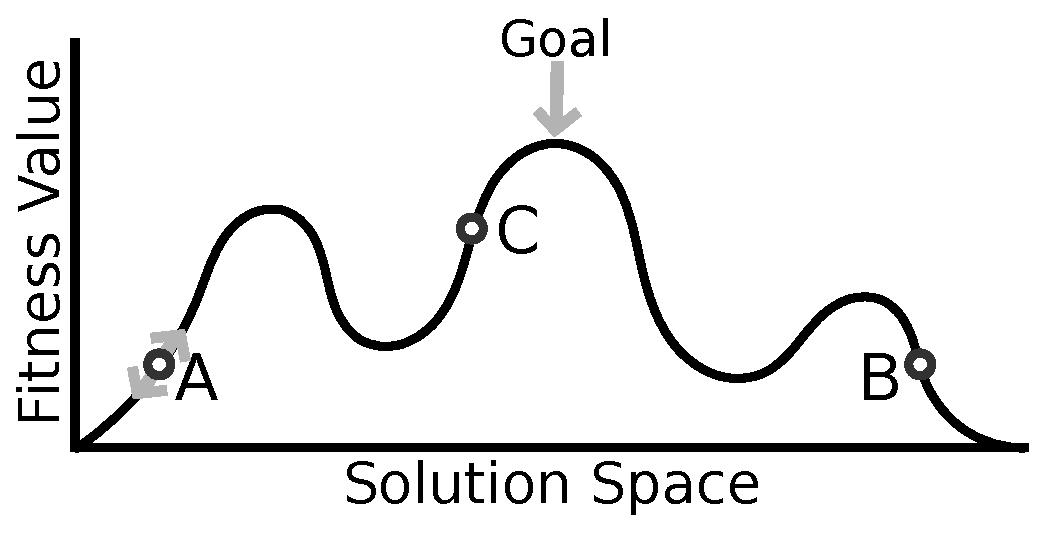
\includegraphics[width=2in]{./pycritters_figs/GeneticAlgStateSpace.eps}}
\afterfig

In the diagram above, {\tt A} and {\tt B} represent randomly generated
individuals with relatively low fitness values. During breeding, there is a
chance that a trait is mutated. This usually results in a lower fitness value,
but can at times be beneficial, as the arrows around {\tt A}
indicate.\footnote{Depending on the trait being mutated and the degree of
mutation, it is also possible that the resulting solution could lie on a
different hill in the solution space.} Breeding between two individuals
generally involves a {\em crossover} of traits between those individuals, 
with the goal of mixing good behaviors in order to create a new individual 
on a different hill in the solution space. For example, breeding {\tt A} 
and {\tt B} could result in {\tt C} in the diagram above, which is closer 
to the global maximum than either of its parents.
 
\begin{ex}
  Read more about genetic algorithms on wikipedia: 
  \url{http://en.wikipedia.org/wiki/Genetic_algorithm}. List several ways that 
  genotypes in a population could be represented.
\end{ex}

% Could be too much of a leap
\begin{ex}
  Read about the 8 queens problem at \url{wikipedia.org/wiki/8_queens}.
  Try to solve it using a genetic algorithm. Hint: you can represent
  each possible solution as a string where each character is a number
  between 0 and 7.
\end{ex}

\section{A Simple Brain Model}

Karl Sims' creatures were driven by control systems called {\em artificial neural
networks}, directed small world graphs that model the behavior of biological brains and
have been used successfully to perform non-linear data analysis in fields such as
pattern matching and image recognition.
\index{neural networks}

The basic unit of computation in a neural network (NN) is the {\em neuron}, which
roughly corresponds to a logic gate in a CPU. However, while logic gates in 
processors only deal with binary values, nodes in most NNs support real numbers.
As is shown in the example below, every neuron (or node) in a network evaluates a 
function that operates on one or more inputs to produce one or more output values. 
Each edge in the graph has a weight associated with it, which scales the value passed in:
\index{neuron}

\beforefig
\centerline{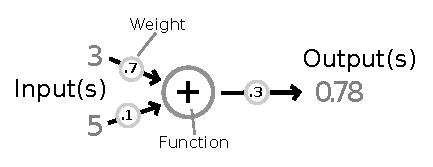
\includegraphics[width=3in]{./pycritters_figs/Neuron.eps}}
\afterfig

In this example of a sum node, the input values {\tt (3,5)} yield 0.78 as the output: 
$(0.7\times 3)+(0.1\times 5) \Rightarrow 2.6$; $2.6 \times 0.3 \Rightarrow 0.78$. 
The function of a given neuron could be any operation on a set of numbers, including 
(but not limited to) difference, product, and sine. More complicated nodes can 
have a memory component.

The simplest type of NN is known as a {\em feed forward} network, which cannot contain cycles and involves {\em hidden} computation layers that act on the values 
of several input nodes and yield values for one or more output nodes:
\index{feed forward neural network}

\beforefig
\centerline{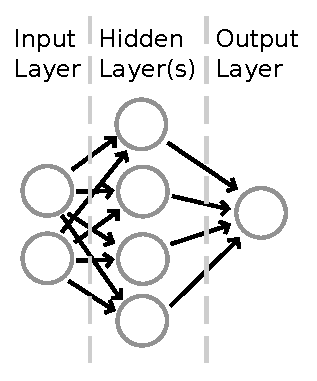
\includegraphics[width=2in]{./pycritters_figs/NN.eps}}
\afterfig

NNs like this can be used effectively for tasks like optical character
recognition (converting handwriting or scanned documents into text). However,
Sims' virtual creatures used more complicted neural networks with no clear
separation between the layers of the network:

\beforefig
\centerline{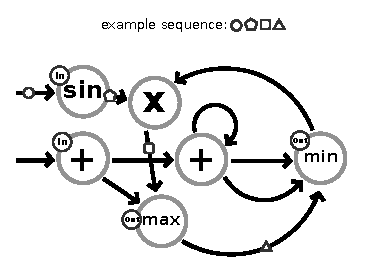
\includegraphics[width=2.5in]{./pycritters_figs/ComplexNN.eps}}
\afterfig

In this example, we follow a sequence of four data elements as they travel 
through the network (obviously, the values change every time they move between 
nodes, but this isn't shown in the diagram). Note that the weights of the edges 
aren't shown and that the second input node's data stream would move in sync 
with the stream that is depicted above. Depending on the implementation of the 
network, edges that have never encountered data before are ignored or assigned a 
value of zero when they propagate data to the nodes.

\section{Body Model}

\section{PyCritters: A Simplified Implementation}

\TODO{Discussion of Results}

\section{The Blind Watchmaker}

As we have seen, complicated systems do not necessarily need to be designed that
way; great complexity (such as that seen in Karl Sim's virtual creatures and in the pycritters) 
can arise from simple processes. This is a counter point to the {\em watchmaker
argument} made famous by the philosopher William Paley in 1802. 
\index{Paley, William}
\index{Watchmaker argument}

The argument follows this basic
framework\footnote{\url{wikipedia.org/wiki/Watchmaker_analogy}}:

\begin{enumerate}
  \item Watches are complex, and if you saw one, you would know that it was made
  by an {\em intelligent designer}, a watchmaker.

  \item {\tt X}, just like a watch, is complex, where {\tt X} is an organ, a
  creature, or anything else. Therefore, it too was created by
  an intelligent designer.
\end{enumerate}

Evolutionary biologist Richard Dawkins refuted this argument in his 1986 book
{\em The Blind Watchmaker: Why the Evidence of Evolution Reveals a Universe
without Design}, in which he used the mammalian eye as an example of a complex
system that could plausibly be the product of natural selection rather than the
result of intelligent design.
\index{Blind Watchmaker@{\em The Blind Watchmaker: Why the Evidence of Evolution Reveals a Universe without Design}}
\index{Dawkins, Richard}

To further prove his point, Dawkins created a computer simulation of {\em
biomorphs}, two dimensional shapes that ``evolved'' based on user selected
mutations.\footnote{\url{wikipedia.org/wiki/The_Blind_Watchmaker}}
\index{Biomorphs}

Karl Sims' virtual creatures can be viewed as a more convincing extension of this early work by
Dawkins, because it doesn't require user interaction to create complex behavior.

\begin{ex}
  Find one of the open source implementations of Dawkins' original Biomorphs
  program, which is called {\em The Blind Watchmaker}, like his book. Can you create 
  seemingly complex shapes with it? If you have time, try to automate the selection process
  by modifying the source code. 
\end{ex}


\printindex

\clearemptydoublepage

%\blankpage
%\blankpage
%\blankpage


\end{document}
